% Build: `pdflatex main` gives the working draft (system named OpenZTAC);
%        `pdflatex main_anon` (which defines \ANON) gives the double-blind submission.
\ifdefined\ANON
  \documentclass[sigconf,review,anonymous]{acmart}
\else
  \documentclass[sigconf,review]{acmart}
\fi

\settopmatter{printacmref=false}
\setcopyright{none}
\renewcommand\footnotetextcopyrightpermission[1]{}
\acmConference[SACMAT '27]{The 32nd ACM Symposium on Access Control Models and Technologies}{July 19--21, 2027}{Durham, UK}

\usepackage{booktabs}
\usepackage{multirow}
\usepackage{tabularx}
\usepackage{colortbl}
\usepackage{graphicx}
\usepackage{tikz}
\usetikzlibrary{positioning,fit,backgrounds,arrows.meta,calc,shapes.multipart,shapes.geometric,decorations.pathreplacing}
\usepackage[ruled,linesnumbered,vlined]{algorithm2e}
\SetAlFnt{\small}
\SetAlCapFnt{\small}
\usepackage{xspace}
\usepackage{enumitem}
\usepackage{pifont}

\setlength{\emergencystretch}{2em}
\newif\ifanon
\ifdefined\ANON \anontrue \else \anonfalse \fi
% Name of our system: anonymised in the submission build only.
\ifanon
  \newcommand{\sysname}{\textsc{Atrium}\xspace}
\else
  \newcommand{\sysname}{\textsc{OpenZTAC}\xspace}
\fi
\newcommand{\chain}{\textsc{Chain-9}\xspace}
\newcommand{\Pc}{P_{\mathrm{class}}}
\newcommand{\Px}{P_{\mathrm{ctx}}}
\newcommand{\Po}{P_{\mathrm{own}}}
\newcommand{\ow}{\mathsf{ow}}
\newcommand{\Gasg}{G^{\mathrm{asg}}}
\newcommand{\Gdel}{G^{\mathrm{del}}}
\newcommand{\sameDept}{\mathsf{sameDept}}
\newcommand{\sameDiv}{\mathsf{sameDiv}}
\newcommand{\role}{\mathsf{role}}
\newcommand{\decide}{\mathsf{decide}}
\newcommand{\obs}{\mathsf{obs}}
\newcommand{\allowv}{\mathtt{allow}}
\newcommand{\denyv}{\mathtt{deny}}
\newcommand{\emp}{\mathrm{emp}}
\newcommand{\ev}[1]{\mathsf{#1}}
\newcommand{\Routes}{\mathcal{R}}
\newcommand{\ok}{\ding{51}}
\newcommand{\no}{\ding{55}}
\newcommand{\RQ}[1]{\textbf{RQ#1}}
\newcommand{\answer}[2]{\par\smallskip\noindent\fbox{\parbox{\dimexpr\columnwidth-2\fboxsep-2\fboxrule\relax}{%
\textbf{Answer to RQ#1.} #2}}\par\smallskip}
% Notes for the authors: shown in the working draft, removed from the submission build.
\ifanon \newcommand{\TODO}[1]{} \else \newcommand{\TODO}[1]{\textcolor{red}{[#1]}} \fi

\begin{document}

\title[Beyond the Decision Point]{Beyond the Decision Point:\\
Layered Conformance Checking of a Zero-Trust ABAC System\\ (Extended Version)}

\ifanon
\author{Anonymous Author(s)}
\affiliation{\institution{Anonymous Institution}\country{}}
\else
\author{\TODO{Author names}}
\affiliation{\institution{\TODO{Affiliation}}\country{\TODO{Country}}}
\fi

\begin{abstract}
We designed, built and deployed \sysname, a zero-trust system for attribute-based access control (ABAC). Its
decision point applies a chain of nine rules, and the first rule that matches a request decides. We proved
five properties of this chain and tested the decision point thoroughly. Yet when we examined the running
system as a whole, on isolated local deployments, several of these guarantees did not hold. This paper explains why and turns the lesson
into a method. We check a deployment at three levels: the rules (L1), the stored state that the rules read
(L2), and every path that enforces a decision (L3). We prove that, under assumptions we state in one place,
the three levels together guarantee that every effect is authorized by a committed state at most $\Delta$ old,
and that no two of them are enough. At L1, a syntactic condition on the decision code
and a query to a satisfiability modulo theories (SMT) solver make testing on a finite set of cases complete.
At L2, a theorem predicts how long a revoked or expired permission keeps working when grants are cached. At
L3, probes exercise every request path of an inventory generated from the web framework's routing table, and
check its audit record. In \sysname v1, the decision point matched
its model on all 368{,}640 test cases and provably keeps departments apart. The system around it did not
behave as well: the risk rule never took effect, revoked permissions kept working for up to the cache lifetime
(and a race re-admitted them in 44--53\,\% of our trials), denials were never logged,
and several request paths skipped the decision point; four of our eighteen findings appeared only once we
generated the route inventory from the routing table. The repaired \sysname v2 passes all 57 enforcement checks;
in median latency it is 47\,\% slower on document reads and 32\,\% slower on denied file requests, while for
decisions the difference stays within the noise of our runs.
As a preliminary transfer, we also applied parts of the method to OpenFGA (an open implementation of Google's
Zanzibar model), Cedar's TinyTodo and Backstage RBAC. All three agreed with their documented rules on every case
we sampled; in each, the state level exposed a documented behaviour by which a change of permission takes
effect late or not at all, and our theorem predicts OpenFGA's cache window to within 50\,ms.
\end{abstract}

\ccsdesc[500]{Security and privacy~Access control}
\ccsdesc[300]{Security and privacy~Logic and verification}
\ccsdesc[300]{Security and privacy~Software security engineering}

\keywords{attribute-based access control, zero trust, conformance testing, data independence,
differential testing, SMT, authorization caching, revocation, complete mediation, threat model}

\maketitle

% =====================================================================================
\section{Introduction}
% =====================================================================================

Zero Trust Architecture (ZTA) asks a policy decision point (PDP) to evaluate every request against the
current state of subjects, resources and context \cite{rose2020zta,chandramouli2023sp800207a,kerman2025sp180035}.
Attribute-based access control (ABAC) is the usual policy model \cite{hu2014sp800162,jin2012abac}. There is a
long tradition of verifying such policies: change-impact analysis \cite{fisler2005margrave}, encodings of XACML
and cloud policies for satisfiability modulo theories (SMT) solvers \cite{turkmen2017xacmlsmt,backes2018zelkova},
and anomaly detection \cite{hu2011anomaly}. Most recently, Cedar's authorizer was proved correct in Lean and
tested against its production implementation \cite{cutler2024cedar,disselkoen2024vgd}.

All of these results are about a function, $\decide(q)$. Nobody deploys a function. A deployed system reads
attributes and grants from a database, caches them, enforces decisions at several endpoints, and writes an
audit trail. A property of $\decide$ becomes a property of the system only if three more things hold: the
PDP sees the state that the specification talks about; every path to a protected object goes through the PDP,
which is Saltzer and Schroeder's complete mediation \cite{saltzer1975protection}; and the record of each
decision survives. Everyone assumes these. Few check them, and almost never together.

We learned this on our own system. We designed and built \sysname, an open-source ZTA/ABAC system with a
Python backend of about 16.8\,kLOC (FastAPI, PostgreSQL, Redis), a document service with real-time
collaboration, and a decision point that evaluates a first-applicable chain we call \chain: an administrator rule followed by nine
policies ($P_1$, $\Pc$, $P_2$--$P_6$, $\Px$, $P_7$). We
wrote down seven security invariants, proved five properties of the chain on paper, wrote 140 tests that
cover 95\,\% of the PDP, and deployed it. When we finally checked the running system as a whole, the PDP was
exactly right, and the system was not.

\paragraph{What we propose.} This paper describes the method we ended up with and what it found, in
\sysname and elsewhere. We model a deployment by its runs, that is, by the sequences of requests,
decisions, effects, records and commits it can produce (\S\ref{sec:system}), state a threat model over that system (\S\ref{sec:threat}),
and define conformance at three levels (\S\ref{sec:levels}). At \textbf{L1}, the decision function must agree
with its model and satisfy the requirements. At \textbf{L2$_\Delta$}, it must decide on committed state at
most $\Delta$ old. At \textbf{L3}, every effect on a protected object must be preceded by an allow decision
for the right action, its obligations must be met, and the decision must be recorded durably. We write the
policy chain once, as executable code, and interpret it three ways: as Python booleans for differential
testing, as z3 terms for proofs, and as Cedar policies (Figure~\ref{fig:method}).
Put simply, each level asks one question about the deployment:
\begin{itemize}
\item \textbf{L1, rules:} does the decision code match the rule model, and do the rules satisfy the security
requirements?
\item \textbf{L2, state:} does the decision use up-to-date data, or stale data from the cache?
\item \textbf{L3, enforcement:} does every request path actually ask the decision point, and is every decision
logged?
\end{itemize}
For each level we build an \emph{oracle}, a procedure that decides whether the observed behaviour of the system
is correct.

\paragraph{Questions.} We ask five questions. \RQ1: Can rule-level conformance be established
\emph{completely} by bounded checking, and what does it find in \sysname? \RQ2: What goes wrong between stored
state and decisions, and does our staleness bound predict it? \RQ3: Which enforcement failures escape L1 and
L2? \RQ4: Do our existing tests, and each level's oracle, catch faults at that level? \RQ5: Do the fixes the
method suggests work, what do they cost, and how does \sysname, before and after repair, compare with other
authorization systems: OpenFGA, an open implementation of Google's Zanzibar model, Cedar, and Backstage RBAC?
We state all five questions here and answer each in its own section: \RQ1 in \S\ref{sec:l1}, \RQ2 in
\S\ref{sec:l2}, \RQ3 in \S\ref{sec:l3}, \RQ4 in \S\ref{sec:adequacy} and \RQ5 in \S\ref{sec:rq5}.

\paragraph{What is new.} The ingredients have precedents. Cedar proves an authorizer against a model and tests
the implementation against it \cite{cutler2024cedar,disselkoen2024vgd}; model-based security testing checks
that an application enforces a policy \cite{mouelhi2008models}; ACtest checks what a configuration change does to
an application's access decisions \cite{xiang2025actest}; data independence is classical
\cite{wolper1986,lazic2003semantic}. What we add is, first, a \emph{checked} finite abstraction for ordinary PDP
code: a syntactic criterion that a tool verifies on the code and a coverage query that an SMT solver answers,
which together turn a finite differential test of the real decision code into a complete one. Second, a
layered workflow with contracts for state and enforcement, stated over runs, that compose with the rule level
into an end-to-end guarantee and can each be tested on a running deployment. Third, evidence from a system we
built and then repaired in several rounds, each re-checked by the same oracles, that the failures that matter lie where a verified or exhaustively tested PDP
cannot see them. The data-independence argument itself is classical; our contribution there is to make its
premise checkable on ordinary decision code, not a new theory. Our aim also differs from that of
broken-access-control scanners such as BACScan and BACFuzz \cite{liu2025bacscan,dharmaadi2025bacfuzz}, which
find vulnerabilities without a specification: we check a deployment against stated requirements, and report
both what holds and under which assumptions.

\paragraph{Contributions.}
\begin{itemize}
\item A formal model of \sysname as a labelled transition system, a threat model with seven adversary classes
derived from it, and a running example that we follow through every level (\S\ref{sec:system},
\S\ref{sec:threat}).
\item Definitions of L1, L2$_\Delta$ and L3 conformance over runs, with a composition theorem (the three levels
together give end-to-end conformance) and an independence result (no two give the third)
(\S\ref{sec:levels}, \S\ref{sec:discussion}).
\item Two results that make bounded checking sound rather than merely plausible: a data-independence lemma
under a syntactic criterion that a tool checks on the decision code, and a completeness theorem whose premise
an SMT query checks (\S\ref{sec:method}). The coverage check found two holes in the world space we had been
using.
\item A tight staleness theorem for TTL-cached grants (\S\ref{sec:method}), whose prediction the measured windows
match to within 0.63\,s over 100 trials (\S\ref{sec:l2}), and a freshness result for the versioned cache of v2.
\item An L3 check whose route inventory is generated from the web framework's routing table and swept with
subjects who must be refused; it found four failures that our hand-built inventory had missed (\S\ref{sec:l3}).
\item Eighteen findings on \sysname v1, each backed by a proof, an exhaustive count or a reproduction, and
mutation evidence that the faults that matter most are invisible to rule-level oracles and to our own tests
(\S\ref{sec:l1}--\S\ref{sec:adequacy}).
\item \sysname v2, which passes every oracle and keeps all requirements provable at a measured latency cost, an
exact compilation of first-applicable chains to Cedar, and a comparison of \sysname with OpenFGA, Cedar's
TinyTodo, Backstage RBAC and, from the literature, Zanzibar (\S\ref{sec:rq5}).
\end{itemize}
Every experiment ran on isolated local deployments of frozen versions of \sysname; we make no claim about any
other installation. This is one deep case study of a system we built, with preliminary transfer to three
independent systems (\S\ref{sec:compare}). The artifact, with every script, raw result and survivor
classification, is described in Appendix~\ref{app:artifact}.

% =====================================================================================
\section{Background and Related Work}
\label{sec:related}
% =====================================================================================

\paragraph{ABAC and zero trust.} ABAC decides on subject, object and environment attributes
\cite{hu2014sp800162,jin2012abac}; XACML and NGAC are its standards \cite{oasis2013xacml,ferraiolo2016sp800178}.
ZTA adds per-request evaluation by a PDP and enforcement by policy enforcement points (PEPs)
\cite{rose2020zta,chandramouli2023sp800207a,kerman2025sp180035}. Risk-adaptive models feed a risk estimate
into the decision \cite{cheng2007fuzzymls,ameer2022bluesky}. Temporal models and usage control
\cite{bertino2001trbac,park2004ucon} make validity intervals and \emph{ongoing} authorization first-class. The
second is what breaks at our state level.

\paragraph{Analysing policies and authorizers.} Margrave \cite{fisler2005margrave}, SMT-based XACML analysis
\cite{turkmen2017xacmlsmt}, Zelkova \cite{backes2018zelkova} and anomaly detection \cite{hu2011anomaly} reason
about policies. Cedar \cite{cutler2024cedar,disselkoen2024vgd} goes further and proves its authorizer correct,
then tests the Rust code against the Lean model. That is the closest work to our L1. Its guarantees are,
quite reasonably, relative to the entities the application passes in; how fresh those entities are, and
whether every endpoint asks, is left to the integrator. Work on synthesizing policies with LLMs
\cite{vatsa2025synth,vatsa2026autocedar} also targets the policy itself.

\paragraph{Testing access control.} Policy mutation \cite{martin2007mutation} and model-based security testing
\cite{mouelhi2008models} test policies, or applications against policies. RoleCast \cite{son2011rolecast} and
MACE \cite{monshizadeh2014mace} find missing or inconsistent checks without a specification, and ACtest
\cite{xiang2025actest} tests configuration changes in web applications. The three closest pieces of work differ
from ours in what they take and what they give. Cedar's verification-guided development takes a formal model of
the authorizer and its production code, and differential random testing yields confidence that the two agree on
the entities the application passes in; our L1 takes arbitrary PDP code and a rule model, and yields agreement
on every world once criterion G and coverage hold, plus proofs of the requirements, but it says nothing about a
language implementation as Cedar's proofs do. Model-based security testing derives tests of an application from
a security model and qualifies them by mutating the policy; it treats the application's state as given. ACtest
runs a trimmed copy of a production system before and after a configuration change, reports the requests whose
decision flips, and leaves it to a person to say which flips are wanted; it needs no requirements, but it judges
changes, not a deployment. None of the three addresses the freshness of the state a decision reads, which is our
L2. Closest to our L3 are scanners for broken access control. BACScan \cite{liu2025bacscan} crawls a running web
application as several users, links pages that change data to pages that show it, and replays changes as the
wrong user, judging success by the data the application later shows; BACFuzz \cite{dharmaadi2025bacfuzz} fuzzes
PHP applications with parameters chosen by a language model and judges success by the SQL statements they
cause. Both find routes and fixtures automatically and need no specification, which our L3 does not do; in
return, they report vulnerabilities, while our L3 checks each inventoried route against the decision of a
specified PDP and checks liveness and the audit record as well. The two are complementary: a scanner's findings
are candidate routes and fixtures for our inventory. Our L1 oracle builds on differential
and property-based testing \cite{claessen2000quickcheck,maciver2019hypothesis}. Bounded checking is usually
justified by the small-scope hypothesis \cite{jackson2012alloy}; we replace the hypothesis with a
data-independence argument \cite{wolper1986,lazic2003semantic} that we can check.

\paragraph{Authorization state and its freshness.} SAAM and authorization recycling
\cite{crampton2006saam,wei2008recycling} reuse cached or inferred decisions. Zanzibar \cite{pang2019zanzibar}
stores relation tuples, evaluates them through namespace configurations with userset rewrites, and avoids
the ``new enemy'' problem with snapshot reads at the timestamps carried by consistency tokens (zookies).
OpenFGA \cite{openfga} is an open implementation of that model. We bound staleness for the plain TTL cache that
most applications actually use, show which code paths break the bound, evaluate a versioned-key fix in
Zanzibar's spirit, and measure OpenFGA's own check cache against the bound. Table~\ref{tab:related} compares
what each line of work takes and gives; Table~\ref{tab:compare} in \S\ref{sec:compare} compares the systems.

\begin{table*}[t]
\caption{What each line of work takes, what it inspects and what it gives, by conformance level (L1 rule, L2
state, L3 enforcement). ``--'' means the work does not address the column.}
\label{tab:related}
\footnotesize
\begin{tabularx}{\textwidth}{@{}>{\raggedright\arraybackslash}p{3.3cm}@{\;\;}>{\raggedright\arraybackslash}X@{\;\;}>{\raggedright\arraybackslash}X@{\;\;}>{\raggedright\arraybackslash}X@{\;\;}>{\raggedright\arraybackslash}X@{\;\;}>{\raggedright\arraybackslash}X@{}}
\toprule
Work & Takes & Inspects & State freshness (L2) & Paths to objects (L3) & Gives; completeness \\
\midrule
Margrave \cite{fisler2005margrave}, XACML-SMT \cite{turkmen2017xacmlsmt}, Zelkova \cite{backes2018zelkova} & policies & the policy, not the code that runs it & -- & -- & properties of the policy; complete for the policy language \\
Cedar with VGD \cite{cutler2024cedar,disselkoen2024vgd} & a formal model and the production authorizer & the authorizer & entities supplied by the application & -- & proofs about the model; sampled agreement of code and model \\
Policy mutation \cite{martin2007mutation} & a policy and its tests & the policy & -- & -- & adequacy of the tests \\
Model-based security testing \cite{mouelhi2008models} & a security model & the application, through generated tests & taken as given & derived from the model & tests qualified by mutation \\
RoleCast \cite{son2011rolecast}, MACE \cite{monshizadeh2014mace} & application source; no specification & source code, statically & -- & static analysis & candidate missing or inconsistent checks \\
ACtest \cite{xiang2025actest} & a trimmed production copy and a configuration change & the running application & -- & production requests & decisions that flip, for a person to judge \\
BACScan \cite{liu2025bacscan}, BACFuzz \cite{dharmaadi2025bacfuzz} & a running application and test accounts; no specification & HTTP responses (BACScan); SQL statements (BACFuzz) & -- & crawling; fuzzing & vulnerabilities \\
Zanzibar \cite{pang2019zanzibar} & its own design & -- & snapshot reads at token timestamps & clients call \texttt{Check} & a consistency guarantee by design \\
\textbf{This work} & requirements, a rule model, the PDP code and a running deployment & PDP code (criterion G); the running system & bound $\Delta$ proved and measured & routing-table inventory, manual for non-HTTP paths & proofs and counterexamples; L1 complete under G and coverage; L3 relative to the inventory \\
\bottomrule
\end{tabularx}
\end{table*}

% =====================================================================================
\section{\sysname: Design and Formal Model}
\label{sec:system}
% =====================================================================================

\paragraph{Architecture.} Figure~\ref{fig:system} shows the parts of \sysname that matter for authorization.
An administration interface (PAP) manages subjects, objects, grants and the policy chain. The PDP loads
subject and object attributes from PostgreSQL on every decision and reads assignment and delegation grants
through a Redis cache keyed by (subject, object), with lifetimes of 120\,s and 60\,s. Three PEP endpoints serve
files. A document service and a real-time collaboration server have their own entry points. Decisions go to
an append-intended ledger. We analyse version~1 as frozen at the start of the study. \sysname~v2 is the
repaired version that we built from the findings and describe in \S\ref{sec:rq5}. So that each result can be
read in one place, the running example and the result tables and figures of \S\ref{sec:l1}--\S\ref{sec:adequacy}
show v2 next to v1; the reader can ignore the v2 columns until \S\ref{sec:rq5}.

\begin{figure}[t]
\centering
\begin{tikzpicture}[
  font=\scriptsize, node distance=2mm,
  box/.style={draw, rounded corners=1.5pt, align=center, inner sep=2pt, minimum height=5mm},
  pep/.style={box, fill=blue!6, text width=19mm},
  dp/.style={box, fill=green!8, text width=17mm},
  st/.style={box, fill=orange!10, text width=17mm},
  bad/.style={box, fill=red!8, text width=17mm},
  arr/.style={-{Stealth[length=1.5mm]}, semithick}]
  \node[pep] (a1) {\texttt{/access/decide}};
  \node[pep, below=of a1] (a2) {\texttt{/pep/access}\\(+owner bypass)};
  \node[pep, below=of a2] (a3) {\texttt{/pep/preview}, \texttt{/download}};
  \node[pep, below=of a3] (a4) {\texttt{/documents/\{id\}}};
  \node[pep, below=of a4] (a5) {collab.\ WebSocket};
  \node[dp, right=9mm of a2] (pdp) {\chain PDP};
  \node[box, fill=gray!10, text width=17mm, above=3mm of pdp] (pap) {PAP\\(policies, grants)};
  \node[bad, right=9mm of a4] (dr) {document rules};
  \node[bad, right=9mm of a5] (cr) {connect-time check};
  \node[st, right=7mm of pdp, yshift=4mm] (redis) {Redis grant cache\\$\tau_{\mathrm{asg}}{=}120$\,s, $\tau_{\mathrm{del}}{=}60$\,s};
  \node[st, below=4mm of redis] (pg) {PostgreSQL\\subjects, objects, grants};
  \node[st, below=4mm of pg] (log) {decision ledger};
  \draw[arr] (a1) -- (pdp); \draw[arr] (a2) -- (pdp); \draw[arr] (a3.east) -- (pdp.south west);
  \draw[arr] (a4) -- (dr); \draw[arr] (a5) -- (cr);
  \draw[arr] (pdp) -- (redis); \draw[arr] (redis) -- node[right]{miss} (pg); \draw[arr] (pdp) -- (pg);
  \draw[arr] (pap.east) -| (pg.north west);
  \draw[arr, dashed] (pdp.south east) -- (log);
  \draw[arr] (dr) -- (pg); \draw[arr] (cr.east) -- (pg.south west);
  \begin{scope}[on background layer]
    \node[draw=gray, dashed, inner sep=2pt, fit=(pdp)] (L1) {};
    \node[draw=gray, dashed, inner sep=3pt, fit=(redis)(pg)] (L2) {};
    \node[draw=gray, dashed, inner sep=3pt, fit=(a1)(a5)(dr)(cr)(log)] (L3) {};
  \end{scope}
  \node[anchor=south west, gray] at (L1.south east) {L1};
  \node[anchor=south, gray] at (L2.north) {L2};
  \node[anchor=north east, gray] at (L3.south east) {L3};
\end{tikzpicture}
\caption{\sysname~v1: request paths, decision procedures (green: the \chain PDP; red: hand-written rules) and
state. The document API and the collaboration channel never reach the PDP, and the file endpoints skip it for
object owners.}
\label{fig:system}
\end{figure}

\paragraph{Notation.} $\mathbb{T}$ is the set of time instants (non-negative reals, in seconds), $\mathbb{B}=\{\mathit{true},\mathit{false}\}$
the Booleans, $\mathbb{N}$ the natural numbers, and $2^X$ the set of all subsets of a set $X$. $\bot$ marks an
undefined value and is used for nothing else. $[\varphi]$ is 1 if the condition $\varphi$ holds and 0 otherwise.

\paragraph{Entities and state.} Let $U$, $O$, $A$, $D$ and $V$ be the sets of subjects, objects, actions,
departments and divisions, with $\{\mathit{read},\mathit{write},\mathit{download},\mathit{delete}\}\subseteq A$,
and let $\mathit{IP}$ be the set of network addresses. A delegation request has a status in
\[
\mathit{St}=\{\mathit{pending},\mathit{approved},\mathit{rejected},\mathit{expired},\mathit{revoked}\}.
\]
Clearances and sensitivities are totally ordered,
$C=\{\mathit{normal}\prec\mathit{elevated}\prec\mathit{delegated}\}$ and
$S=\{\mathit{public}\prec\mathit{internal}\prec\mathit{sensitive}\prec\mathit{top\_secret}\}$, and are compared
through the ranks $\kappa_C:C\to\{1,2,3\}$ and $\kappa_S:S\to\{0,1,2,3\}$ of the implementation.

\begin{definition}[State]\label{def:state}
A state $\sigma\in\Sigma$ consists of the attribute functions
$\role:U\to\{\mathrm{adm},\mathrm{dir},\mathrm{dm},\emp,\mathrm{cust}\}$, $\mathsf{dept}:U\cup O\to D$,
$\mathsf{div}:U\cup O\to V\cup\{\bot\}$, $\mathsf{clr}:U\to C$, $\mathsf{sens}:O\to S$, $\mathsf{own}:O\to U$, the
risk inputs $\mathsf{fl}:U\to\mathbb{N}$ (failed logins) and $\mathsf{ip}:U\to\mathit{IP}\cup\{\bot\}$ (last known
address), and two grant relations: assignments $\mathit{Asg}\subseteq U\times O\times 2^A\times\mathbb{T}\times
(\mathbb{T}\cup\{\infty\})\times\mathbb{B}$, whose elements $(u,o,B,t_f,t_u,b)$ give the granted action
set $B\subseteq A$, the validity interval $[t_f,t_u)$ and an active flag $b$; and
delegations $\mathit{Del}\subseteq U\times O\times 2^A\times\mathit{St}\times\mathbb{T}$, whose elements
$(u,o,B,s,t_e)$ give the action set, the status and the expiry $t_e$. It further contains the parts that only
procedures other than the PDP read: the policy store $\mathit{Pol}$, which records for each rule whether the PAP
shows it as active; the document workflow, a status
$\mathsf{wf}:O_{\mathrm{doc}}\to\{\mathit{draft},\mathit{review},\mathit{pending},\mathit{approved},
\mathit{published},\mathit{archived}\}$ and collaborators $\mathit{Col}\subseteq U\times O_{\mathrm{doc}}$ for the
objects $O_{\mathrm{doc}}\subseteq O$ that are documents; the open collaboration sessions
$\mathit{Ses}\subseteq U\times O_{\mathrm{doc}}$; and the ledger $\mathit{Led}$, a sequence of decision records.
\end{definition}

The roles are administrator, director, division manager, employee, and $\mathrm{cust}$ for any custom role
that an administrator created. Grants become sets of actions at time $t$:
\begin{align*}
\Gasg_t(u,o) &= \textstyle\bigcup\{B \mid (u,o,B,t_f,t_u,\mathit{true})\in\mathit{Asg},\ t_f\le t<t_u\},\\
\Gdel_t(u,o) &= \textstyle\bigcup\{B \mid (u,o,B,\mathit{approved},t_e)\in\mathit{Del},\ t<t_e\}.
\end{align*}
The delegation workflow always sets $B=\{\mathit{read}\}$. A request is $q=(u,o,a,c)\in Q=U\times O\times A\times
\mathit{Ctx}$, where the context $c\in\mathit{Ctx}$ carries the hour of day $h(c)$ and the source address
$\mathit{ip}(c)\in\mathit{IP}$. The risk score is
\begin{align*}
\rho(u,c)=\min\bigl(100,\;&30\,[h(c)\notin[7,19)]+40\,[\mathsf{fl}(u)\ge5]\\
&+15\,[2\le\mathsf{fl}(u)\le4]+25\,[\bot\neq\mathsf{ip}(u)\neq\mathit{ip}(c)]\bigr),
\end{align*}
and the threshold is $\theta=70$. We write $\sameDept(u,o)$ for
$\mathsf{dept}(u)=\mathsf{dept}(o)$, $\sameDiv(u,o)$ for $\mathsf{div}(u)\neq\bot\wedge\mathsf{div}(u)=\mathsf{div}(o)$,
and $\sameDiv^\circ$ for plain equality of divisions, under which $\bot=\bot$.

\begin{definition}[Rule chain]\label{def:chain}
A chain is a sequence
\[
\Pi=\langle(r_1,e_1,\gamma_1),\dots,(r_n,e_n,\gamma_n)\rangle
\]
of rule names $r_i$, effects $e_i\in\{\allowv,\denyv\}$ and guards $\gamma_i:\Sigma\times\mathbb{T}\times Q\to\mathbb{B}$,
with $\gamma_n\equiv\mathit{true}$ so that some rule always applies.
Its first-applicable semantics is
\[
\decide^\Pi_{\sigma,t}(q)=\bigl(e_k,r_k\bigr)\quad\text{where}\quad k=\min\{i\mid\gamma_i(\sigma,t,q)\}.
\]
\end{definition}

\chain is the chain of Table~\ref{tab:chain}. The administrator rule has no documented priority; it is
implemented as a bypass before the chain, which is the same thing as a first rule.

\begin{table}[t]
\caption{\chain as implemented in v1, first-applicable from top to bottom. $\pi$ is the documented priority.}
\label{tab:chain}
\small
\begin{tabular}{@{}l@{\;}r@{\;}l@{\;}l@{}}
\toprule
Rule & $\pi$ & Eff. & Guard (for $q=(u,o,a,c)$ at time $t$) \\
\midrule
Admin & -- & allow & $\role(u)=\mathrm{adm}$ \\
$P_1$ & 10 & deny & $\neg\sameDept\wedge\Gdel_t(u,o)=\emptyset$ \\
$\Pc$ & 15 & deny & $\kappa_S(\mathsf{sens}(o))>0\wedge\kappa_C(\mathsf{clr}(u))<\kappa_S(\mathsf{sens}(o))$ \\
 & & & $\;\wedge\neg(\mathrm{dir}\wedge\sameDept)\wedge\neg(\mathrm{dm}\wedge\sameDept\wedge\sameDiv^\circ)$ \\
$P_2$ & 20 & allow & $\role(u)=\mathrm{dir}\wedge\sameDept$ \\
$P_3$ & 30 & allow & $\role(u)=\mathrm{dm}\wedge\sameDept\wedge\sameDiv^\circ$ \\
$P_4$ & 40 & allow & $\role(u)\in\{\emp,\mathrm{dm}\}\wedge a\in\Gasg_t(u,o)$ \\
$P_5$ & 45 & deny & $\role(u)=\emp\wedge\Gasg_t(u,o)=\emptyset$ \\
$P_6$ & 50 & allow & $a\in\Gdel_t(u,o)$ \\
$\Px$ & 60 & deny & $\rho(u,c)\ge\theta$ \\
$P_7$ & 99 & deny & $\mathit{true}$ \\
\bottomrule
\end{tabular}
\end{table}

\paragraph{Routes and runs.} The PDP is one of several components that decide. We therefore model the
whole deployment as a labelled transition system: a system state is the committed state together with the
requests in progress, and each transition is labelled by one event. We only need the sequences of labels,
which we call runs. Figure~\ref{fig:run} shows a run and what each conformance level of \S\ref{sec:levels}
will constrain in it.

\begin{definition}[Routes]\label{def:routes}
A route $r\in\Routes$ is an externally reachable operation, given by a decision procedure
$D_r:\Sigma\times\mathbb{T}\times Q\to\{\allowv,\denyv\}$; an action map $\alpha_r:A\cup\{\bot\}\to A$ that gives
the action the procedure evaluates, from the route and possibly from an action $a_c$ sent by the client ($\bot$
if none); a set of obligations $\mathit{Ob}_r$ (such as multi-factor authentication); and an effect: returning
content of $o$ or changing $\sigma$.
\end{definition}

\begin{definition}[Runs]\label{def:runs}
A run is a finite sequence of timestamped events of six kinds, each tagged with the identifier $k$ of the request
it belongs to: $\ev{req}_k(r,u,o,a_c,c)$, a client request on route $r$ by an authenticated principal $u$;
$\ev{dec}_k(u,o,a,d)$, a decision $d$ by some decision procedure;
$\ev{eff}_k(r,u,o,a)$, an effect (content returned, or state changed) on behalf of $u$;
$\ev{rec}(e)$, the durable commit of a record of decision event $e$;
$\ev{com}_k(\Delta\sigma)$, the commit of a state change made by request $k$; and
$\ev{resp}_k$, the response that ends request $k$. Expiry needs no event: it is a function of time. The
committed state $\sigma_t$ is the result of applying, in order, every $\ev{com}$ event with timestamp at most $t$
to an initial state $\sigma_0$. A run is \emph{complete} if every request in it has a response. A run is
\emph{well-formed} if (W1) each request identifier $k$ has exactly one $\ev{req}_k$, which precedes every other
event tagged $k$, and at most one $\ev{resp}_k$, which follows every $\ev{dec}_k$, $\ev{eff}_k$ and $\ev{com}_k$;
(W2) every $\ev{com}_k$ that changes state is preceded, in request $k$, by an $\ev{eff}_k$ for that change, so a
state change, including a change of grants, is an effect that takes hold at its commit; and (W3) every $\ev{rec}(e)$ follows the decision event $e$ it
records. We consider well-formed runs only; the event logs of a web server with one transaction per request,
such as \sysname, have this shape.
\end{definition}

In v1, $D_r$ is the \chain PDP for the decision API and for non-owners on the file endpoints. For owners it
is a constant $\allowv$; for the document API it is a set of hand-written workflow rules; and for the
collaboration channel it is a connect-time check. Figure~\ref{fig:system} draws these four procedures.

\begin{figure}[t]
\centering
\begin{tikzpicture}[font=\scriptsize, >={Stealth[length=1.4mm]}, x=0.86cm,
  ev/.style={circle, draw, inner sep=1.4pt},
  br/.style={decorate, decoration={brace, amplitude=3pt, mirror}, semithick}]
  \node[anchor=east, align=right] at (0,1.1) {admin};
  \node[anchor=east, align=right] at (0,0) {request\\of $u$};
  \draw[gray!60] (0,1.1) -- (7.7,1.1);
  \draw[gray!60] (0,0) -- (7.7,0);
  \node[ev, fill=orange!50] (c1) at (0.7,1.1) {}; \node[above=1pt] at (c1) {$\ev{com}(\Delta\sigma_1)$};
  \node[ev, fill=orange!50] (c2) at (4.9,1.1) {}; \node[above=1pt] at (c2) {$\ev{com}(\Delta\sigma_2)$};
  \node[ev, fill=blue!40] (rq) at (1.2,0) {}; \node[below=1pt] at (rq) {$\ev{req}(r,u,o,a_c,c)$};
  \node[ev, fill=green!50] (dc) at (3.3,0) {}; \node[below=1pt] at (dc) {$\ev{dec}(u,o,a,d)$};
  \node[ev, fill=red!50] (ef) at (5.5,0) {}; \node[below=1pt] at (ef) {$\ev{eff}(r,u,o,a)$};
  \node[ev, fill=gray!50] (rc) at (7.3,0) {}; \node[below=1pt] at (rc) {$\ev{rec}(e)$};
  \draw[->, dashed, green!40!black] (dc) -- (2.3,1.03);
  \node[font=\tiny, green!40!black, anchor=east] at (2.62,0.55) {reads $\sigma_{t'}$};
  \node[font=\tiny, green!40!black, align=left, anchor=west] at (3.2,0.55) {L1: $d=\mathcal{M}(\sigma_{t'},t',q)$\\L2$_\Delta$: $t'\ge t-\Delta$};
  \draw[br] (3.3,-0.42) -- node[below=3pt, font=\tiny]{L3: an allow for $\alpha_r$ and its obligations come first} (5.5,-0.42);
  \draw[br] (3.3,-0.95) -- node[below=3pt, font=\tiny]{L3: the decision is recorded, whatever the outcome} (7.3,-0.95);
  \draw[->, gray] (0,-1.55) -- (7.8,-1.55) node[right]{time};
\end{tikzpicture}
\caption{A run: one request (lower line) interleaved with administrative commits (upper line). The decision
at time $t$ reads the committed state $\sigma_{t'}$. Each level of \S\ref{sec:levels} constrains a different part
of the run: L1 the value of the decision, L2$_\Delta$ how old the state it reads may be, and L3 what must
precede the effect and follow the decision.}
\label{fig:run}
\end{figure}

\subsection{Running Example}
\label{sec:example}

Figure~\ref{fig:example} shows a small organisation that we use throughout. Department \emph{Finance} has the
divisions \emph{Accounting} and \emph{Audit}; department \emph{Legal} has \emph{Compliance}. Ana is an
employee in Accounting with \emph{normal} clearance, Dan manages Audit, and Lea directs Legal. Object $r$ is
an \emph{internal} Accounting report and $o$ an \emph{internal} Legal contract.
\begin{itemize}
\item[(a)] Ana is assigned $\{\mathit{read}\}$ on $r$ and reads it. $P_4$ allows, in v1 and in v2.
\item[(b$_1$)] Dan asks to write $o$. $P_1$ denies, since he is in another department and holds no delegation.
\item[(b$_2$)] Lea now assigns Dan $\{\mathit{read},\mathit{write}\}$ on $o$ and approves his request for a
read-only delegation. In v1 the write passes $P_1$, because a delegation now exists, then $\Pc$, $P_2$ and
$P_3$, and is allowed by $P_4$; \S\ref{sec:l1} shows that this happens in general. In v2, $P_4$ also requires $\sameDept$, the
delegation does not contain \emph{write}, and $P_7$ denies.
\item[(c$_1$)] Ana, unassigned, requests $r$ at 02:00 after five failed logins, so
$\rho=30+40=70\ge\theta$. In v1, $P_5$ denies.
\item[(c$_2$)] Had she been assigned, v1 would have allowed her through $P_4$, and the risk rule would never
have been consulted; \S\ref{sec:l1} proves that this is always so. In v2, $\Px$ is evaluated first and denies both (c$_1$) and
(c$_2$).
\end{itemize}
The v2 column previews the repaired chain $\mathcal{F}$ of \S\ref{sec:rq5}. We computed the traces in
Figure~\ref{fig:example} by evaluating both chains with the reference semantics described in \S\ref{sec:method};
\S\ref{sec:l1} shows that this semantics agrees with the PDP code on every world.

\begin{figure*}[t]
\centering
\begin{minipage}[c]{0.43\textwidth}
\centering
\begin{tikzpicture}[font=\scriptsize, node distance=3mm,
  dept/.style={draw, rounded corners=2pt, fill=blue!8, minimum width=15mm, align=center, inner sep=2pt},
  div/.style={draw, rounded corners=2pt, fill=gray!10, minimum width=15mm, align=center, inner sep=2pt},
  subj/.style={draw, circle, fill=yellow!20, inner sep=0.5pt, minimum size=8mm, align=center},
  obj/.style={draw, fill=orange!12, align=center, inner sep=2pt},
  arr/.style={-{Stealth[length=1.4mm]}, semithick}]
  \node[dept] (fin) at (0,0) {Finance};
  \node[dept] (leg) at (4.6,0) {Legal};
  \node[div] (acc) at (-0.9,-1.0) {Accounting};
  \node[div] (aud) at (1.0,-1.0) {Audit};
  \node[div] (com) at (4.6,-1.0) {Compliance};
  \draw (fin) -- (acc); \draw (fin) -- (aud); \draw (leg) -- (com);
  \node[subj] (ana) at (-1.4,-2.3) {Ana\\$\emp$};
  \node[subj] (dan) at (1.0,-2.3) {Dan\\dm};
  \node[subj] (lea) at (4.0,-2.3) {Lea\\dir};
  \node[obj] (r) at (-0.2,-3.6) {$r$: report\\internal};
  \node[obj] (o) at (3.0,-3.6) {$o$: contract\\internal};
  \draw[gray] (acc) -- (ana); \draw[gray] (aud) -- (dan); \draw[gray] (com) -- (lea);
  \draw[gray] (acc) -- (r); \draw[gray] (com) -- (o);
  \draw[arr, teal] (ana) -- node[left, pos=0.4]{asg \{read\} (a)} (r);
  \draw[arr, purple] (dan) -- node[above, sloped, pos=0.5]{asg \{read, write\}} (o);
  \draw[arr, purple, dashed] (dan.south east) to[bend right=25] node[below, sloped, pos=0.55]{del \{read\}} (o.west);
  \draw[arr, gray, dotted] (lea) -- node[right, pos=0.3]{grants (b$_2$)} (o);
  \node[align=left, anchor=north west, text width=66mm] at (-1.9,-4.3)
    {Ana: \emph{normal} clearance. (c): 02:00, five failed logins, $\rho=70$.};
\end{tikzpicture}
\end{minipage}%
\hfill
\begin{minipage}[c]{0.55\textwidth}
\centering\scriptsize
\begin{tabular}{@{}l@{\;}ccccc@{}}
\toprule
\multicolumn{6}{@{}l}{v1 (\chain)} \\
\midrule
rule & (a) & (b$_1$) & (b$_2$) & (c$_1$) & (c$_2$) \\
\midrule
Admin & $\cdot$ & $\cdot$ & $\cdot$ & $\cdot$ & $\cdot$ \\
$P_1$ & $\cdot$ & \cellcolor{red!20}\textbf{deny} & $\cdot$ & $\cdot$ & $\cdot$ \\
$\Pc$ & $\cdot$ &  & $\cdot$ & $\cdot$ & $\cdot$ \\
$P_2$ & $\cdot$ &  & $\cdot$ & $\cdot$ & $\cdot$ \\
$P_3$ & $\cdot$ &  & $\cdot$ & $\cdot$ & $\cdot$ \\
$P_4$ & \cellcolor{green!20}\textbf{allow} &  & \cellcolor{green!20}\textbf{allow} & $\cdot$ & \cellcolor{green!20}\textbf{allow} \\
$P_5$ &  &  &  & \cellcolor{red!20}\textbf{deny} &  \\
$P_6$ &  &  &  &  &  \\
$\Px$ &  &  &  &  &  \\
$P_7$ &  &  &  &  &  \\
\bottomrule
\end{tabular}%
\hspace{3mm}%
\begin{tabular}{@{}l@{\;}ccccc@{}}
\toprule
\multicolumn{6}{@{}l}{v2 ($\mathcal{F}$)} \\
\midrule
rule & (a) & (b$_1$) & (b$_2$) & (c$_1$) & (c$_2$) \\
\midrule
Admin & $\cdot$ & $\cdot$ & $\cdot$ & $\cdot$ & $\cdot$ \\
$\Px$ & $\cdot$ & $\cdot$ & $\cdot$ & \cellcolor{red!20}\textbf{deny} & \cellcolor{red!20}\textbf{deny} \\
$P_1$ & $\cdot$ & \cellcolor{red!20}\textbf{deny} & $\cdot$ &  &  \\
$\Pc$ & $\cdot$ &  & $\cdot$ &  &  \\
$P_2$ & $\cdot$ &  & $\cdot$ &  &  \\
$P_3$ & $\cdot$ &  & $\cdot$ &  &  \\
$\Po$ & $\cdot$ &  & $\cdot$ &  &  \\
$P_4$ & \cellcolor{green!20}\textbf{allow} &  & $\cdot$ &  &  \\
$P_6$ &  &  & $\cdot$ &  &  \\
$P_5$ &  &  & $\cdot$ &  &  \\
$P_7$ &  &  & \cellcolor{red!20}\textbf{deny} &  &  \\
\bottomrule
\end{tabular}%

\end{minipage}
\caption{Running example. Left: organisation, subjects (role), objects (sensitivity) and grants. Right: rule-by-rule
evaluation of each case in v1 (\chain) and v2 (the repaired chain $\mathcal{F}$); $\cdot$ marks a guard that is
false, the coloured cell the first applicable rule, and blank cells rules that are never reached. Cases:
(a) Ana reads $r$; (b$_1$) Dan writes $o$; (b$_2$) the same after Lea's grants; (c$_1$) Ana, unassigned, reads $r$
under high risk; (c$_2$) the same with an assignment.}
\label{fig:example}
\end{figure*}

\paragraph{Our design specification.} Before this study we had formalized the chain in a design document,
with three differences from the code that define $\mathcal{S}_{\mathrm{doc}}$: (D1) $P_4$ requires
$a=\mathit{read}\wedge\Gasg_t\neq\emptyset$; (D2) $P_3$ and $\Pc$ use $\sameDiv$; (D3) clearance is typed as a
sensitivity, which we resolve with the implementation's ranks. The document proves five properties, among them
an employee least-privilege theorem (LP in Table~\ref{tab:req}).

\paragraph{Requirements.} Table~\ref{tab:req} lists eight requirements, each a predicate $\phi(\sigma,t,q,d)$
over a state, a request and a decision. Since we audit our own system, a reader may reasonably worry that we
chose requirements it fails. To guard against that, we took every requirement word for word from text we had
written before the study: the ``hard invariants'' in our developer guide, the policy descriptions the PAP
displays, and the design document. Appendix~\ref{app:prov} quotes each source. Our own documents disagree in
four places, and as the system's designers we resolved each disagreement ourselves; no separate policy owner
exists for \sysname. We give the reason for each choice and, where it matters, the verdicts under the other
reading. (C1) The invariant ``[employee] access $\leftrightarrow$ assigned or delegated'' gives R4, but $P_5$'s
description denies every unassigned employee. (C2) $\Px$'s description says it ``denies access when the
computed risk score \ldots{} meets or exceeds the configured threshold'' (R6), but the design document places it
after every allow rule. (C3) The developer guide gives the order in which access is decided as ``Admin $\to$
Owner $\to$ Cross-dept+no-delegation $\to$ \ldots'', so an owner may open her own object, yet the invariant on
employee access and $\Pc$'s description name no owner. We follow the statements we had labelled as invariants,
and \S\ref{sec:l1} reports the other readings of C1 and C2. For C3 we keep both statements and read the owner
rule as a narrow exception: an owner may read and download her object, which is what ``opening'' it means,
and only inside her department, because the isolation invariant (R1) has no exception at all. (C4) The
developer guide gives $P_4$ as ``\ldots{} $\wedge$ action=read $\Rightarrow$ allow'' and describes employees as
``read-only on assigned resources within their division'', and the design document says that ``assignments grant read access only,
never write''; $P_4$'s description in the PAP grants access ``only for actions included in the assignment''.
Two documents, one of them the guide, against one: we read assignments as granting read only, which makes the
design document's least-privilege theorem (LP) a requirement, with the owner exception of C3.

\begin{table}[t]
\caption{Requirements, for $\role(u)\neq\mathrm{adm}$, and the documents they come from, all written before the
study (G: developer guide; S: policy descriptions shown by the PAP; M: design document). Appendix~\ref{app:prov}
quotes each source; \S\ref{sec:l1} gives the verdicts. $\ow$ is the owner exception of C3. LP comes from the
design document's theorem, which has no owner exception; with C4 it is a requirement.}
\label{tab:req}
\small
\begin{tabularx}{\columnwidth}{@{}l@{\;}>{\raggedright\arraybackslash}X@{\;}l@{}}
\toprule
 & Requirement & Source \\
\midrule
R1 & $\neg\sameDept\wedge\Gdel_t=\emptyset\Rightarrow\denyv$ (isolation) & G, S \\
R2 & $\mathsf{cls}(u,o)\wedge\neg\ow\Rightarrow\denyv$ (classification) & S, G \\
R3 & $\emp\wedge\allowv\Rightarrow a\in\Gasg_t\cup\Gdel_t\vee\ow$ (need-to-know) & G, S \\
R4 & $\emp\wedge a\in\Gdel_t\wedge\rho<\theta\wedge\neg\mathsf{cls}\Rightarrow\allowv$ (delegation suffices) & G \\
R5 & $\neg\sameDept\wedge\allowv\Rightarrow a\in\Gdel_t$ (cross-dept.\ only via delegation) & G \\
R6 & $\rho\ge\theta\Rightarrow\denyv$ (risk) & S \\
R7 & $\allowv\Rightarrow(\mathrm{dir}\wedge\sameDept)\vee(\mathrm{dm}\wedge\sameDept\wedge\sameDiv)\vee((\emp\vee\mathrm{dm})\wedge a\in\Gasg_t)\vee a\in\Gdel_t\vee\ow$ (every allow within an allow rule's scope) & S, G \\
\midrule
LP & $\emp\wedge\sameDept\wedge\Gdel_t=\emptyset\wedge\allowv\Rightarrow(a=\mathit{read}\wedge\Gasg_t\neq\emptyset)\vee\ow$ (employee least privilege) & M, G \\
\bottomrule
\end{tabularx}
\end{table}

Here $\mathsf{cls}(u,o)$ is $\Pc$'s guard with $\sameDiv$ in place of $\sameDiv^\circ$, and
\[
\ow(u,o,a)\equiv\mathsf{own}(o)=u\wedge\sameDept(u,o)\wedge a\in\{\mathit{read},\mathit{download}\}
\]
is the owner exception of C3. We write $R$ for the set $\{\mathrm{R1},\dots,\mathrm{R7},\mathrm{LP}\}$, and $\mathcal{M}$ for
\chain read as a reference model. The v1 PDP never reads $\mathsf{own}$ (its owner rule sits outside it,
\S\ref{sec:system}), so the exception changes none of its verdicts; we checked this by repeating every L1 run.

% =====================================================================================
\section{Threat Model}
\label{sec:threat}
% =====================================================================================

A zero-trust system is supposed to hold up against its own users. We therefore model an insider, and we
state precisely what the adversary can do and what counts as a successful attack, because the three
conformance levels are defined against exactly these goals.

\paragraph{Assets.} The protected assets are (i) the content of objects, including documents in every
workflow state; (ii) the grant relations $\mathit{Asg}$ and $\mathit{Del}$, since whoever can change them can
change future decisions; and (iii) the decision ledger, which an investigator needs in order to reconstruct who
was allowed and who was refused.

\paragraph{Trusted base.} We trust the administrators (role $\mathrm{adm}$) and the PAP they use, the database,
the cache, the deployed server code and its configuration, and the transport (TLS). Trusting the code means
we assume the server executes what is in the repository; it does not mean we assume the code is correct,
which is what the three levels test. A compromised administrator or database can grant anything, and no
check on the decision logic can detect that.

\begin{definition}[Adversary]\label{def:adv}
The adversary $\mathcal{A}$ controls a set $U_{\mathcal{A}}\subseteq U$ of principals with
$\role(u)\neq\mathrm{adm}$, and holds valid credentials (tokens and sessions) for them. $\mathcal{A}$ has four
capabilities.
\begin{description}
\item[Cap1, requests.] For any $r\in\Routes$, $u\in U_{\mathcal{A}}$, $o\in O$ and $a_c\in A\cup\{\bot\}$,
$\mathcal{A}$ can emit $\ev{req}(r,u,o,a_c,c)$, choosing every field of $c$ that the client controls (body,
headers, query parameters). Server-derived context (time, failed-login count) is not under its control.
\item[Cap2, scheduling.] $\mathcal{A}$ chooses when its requests are sent, including concurrently with any other
principal's requests and transactions, such as an administrator's revocation. It does not control the server's
scheduler.
\item[Cap3, persistence.] Credentials and open sessions issued to $u\in U_{\mathcal{A}}$ stay with $\mathcal{A}$
until they expire. Revoking a grant does not revoke them.
\item[Cap4, workflow.] $\mathcal{A}$ can use every legitimate workflow open to $u$: request delegations, create
and own objects, edit drafts, accept collaboration invitations. Changes that only administrators make, such as
moving $u$ to another department, are not under its control, but it benefits from them.
\end{description}
\end{definition}

\begin{definition}[Attack goals]\label{def:goals}
Let $\Delta^\ast\ge0$ be the staleness that the operator tolerates. A run is an \emph{attack} if it contains
one of the following.
\begin{description}
\item[G1, unjustified effect.] An event $\ev{eff}(r,u,o,a)$ at $t$ with $u\in U_{\mathcal{A}}$ such that
$\mathcal{M}$ denies $(u,o,a,c)$ in $\sigma_{t'}$ for every $t'\in[t-\Delta^\ast,t]$.
\item[G2, requirement violation.] An $\allowv$ for a request $q$ of $u\in U_{\mathcal{A}}$ at $t$ and some
$\phi\in R$ with $\neg\phi(\sigma_{t'},t',q,\allowv)$ for every $t'\in[t-\Delta^\ast,t]$.
\item[G3, unrecorded decision.] A decision event $e$ of request $k$ of some $u\in U_{\mathcal{A}}$ such that
$\ev{resp}_k$ occurs and is not preceded by $\ev{rec}(e)$.
\item[G4, lingering access.] A G1 effect whose only justification in $\mathcal{M}$ was a grant that ended (by
revocation or expiry) before $t-\Delta^\ast$.
\item[G5, unauthorised administration.] A $\ev{com}$ that changes $\mathit{Asg}$ or $\mathit{Del}$ on behalf
of $u\in U_{\mathcal{A}}$ when the administrative policy $\Pi_{\mathrm{adm}}$ (approver, owner, the object's
director, or an administrator) does not authorise $u$.
\end{description}
\end{definition}

G1 and G2 are \emph{historical}: a request is attacked only if no committed state of the last $\Delta^\ast$
justifies it. With caching, no $\Delta^\ast>0$ can promise more, since a grant may end between the state a
decision reads and the decision itself; a current-state guarantee needs synchronous reads. G2 differs from G1
because the model itself may allow the request, and the fault lies in the model. G2 concerns allows only;
R4, which demands an allow, is checked at L1 but is a matter of availability, not an attack goal. G3 matters
because a silently refused prober leaves nothing for an investigator to find.

\paragraph{Out of scope.} Compromise of the trusted base; injection and cross-site attacks on the web
front end; denial of service; side channels; and social engineering. The collaboration server's protocol is in
scope only through its authorization check.

\paragraph{Adversary classes.} Table~\ref{tab:adv} groups the attacks open to $\mathcal{A}$ into seven classes,
according to what the adversary exploits. Each class uses a subset of Cap1--Cap4, reaches one of G1--G5, and has a
\emph{primary} level, the one whose oracle observes it on its own; attacks can combine classes, as a lingering
grant used through a bypass does (Figure~\ref{fig:threat}). We arrived at these classes while analysing v1; the evaluation (\S\ref{sec:eval}) gives a
concrete instance of each, and Table~\ref{tab:findings} at the end of \S\ref{sec:l3} maps every finding to its
class. Figure~\ref{fig:threat} shows where each class enters the system. The mapping already contains our main point:
only A1 is visible to an oracle that tests the decision function.

\begin{table}[t]
\caption{Adversary classes, with the capabilities they use, the goal they reach, and their primary level, whose
oracle observes them on its own.}
\label{tab:adv}
\small
\begin{tabularx}{\columnwidth}{@{}l@{\;}X@{\;}l@{\;}l@{\;}l@{}}
\toprule
 & Class & Cap. & Goal & Lvl \\
\midrule
A1 & over-privileged insider: the chain itself allows too much & Cap1, Cap4 & G2 & L1 \\
A2 & lingering grantee: keeps using a revoked or expired grant & Cap1, Cap3 & G4 & L2 \\
A3 & racer: decides concurrently with a revocation & Cap2 & G4 & L2 \\
A4 & path shopper: picks a route or action the PDP does not see & Cap1 & G1 & L3 \\
A5 & owner and mover: uses ownership, also after leaving the department & Cap1, Cap4 & G1 & L3 \\
A6 & silent prober: probes objects, denials leave no record & Cap1 & G3 & L3 \\
A7 & unauthorised revoker: removes other people's grants & Cap1 & G5 & L3 \\
\bottomrule
\end{tabularx}
\end{table}

\begin{figure}[t]
\centering
\begin{tikzpicture}[font=\scriptsize, node distance=2mm,
  box/.style={draw, rounded corners=1.5pt, align=center, inner sep=1.5pt, minimum height=4.6mm},
  rt/.style={box, fill=blue!6, text width=18mm},
  tb/.style={box, fill=green!8, text width=15mm},
  adv/.style={draw, fill=red!10, rounded corners=2pt, align=center, text width=10mm, minimum height=26mm},
  att/.style={-{Stealth[length=1.4mm]}, red!70!black, semithick},
  lv/.style={font=\tiny\bfseries, fill=white, inner sep=0.6pt}]
  \node[adv] (A) at (0,0) {$\mathcal{A}$\\$U_{\mathcal{A}}$\\(Cap1--Cap4)};
  \node[rt] (r1) at (2.4,1.45) {decision API};
  \node[rt, below=of r1] (r2) {file endpoints};
  \node[rt, below=of r2] (r3) {document API};
  \node[rt, below=of r3] (r4) {collab.\ channel};
  \node[rt, below=of r4] (r5) {grant routes};
  \node[tb] (pdp) at (5.2,0.9) {PDP (\chain)};
  \node[tb, below=3mm of pdp] (cache) {grant cache};
  \node[tb, below=3mm of cache] (db) {database};
  \node[tb, below=3mm of db] (led) {ledger};
  \node[tb, above=3mm of pdp] (adm) {administrators, PAP};
  \begin{scope}[on background layer]
    \node[draw=green!50!black, dashed, thick, rounded corners=3pt, inner sep=2.5pt, fit=(adm)(pdp)(cache)(db)(led), label={[font=\tiny, green!40!black]below:trusted base}] (T) {};
  \end{scope}
  \foreach \i in {1,...,5} \draw[att] (A.east) -- (r\i.west);
  \draw[-{Stealth[length=1.2mm]}, gray] (r1.east) -- (pdp.west);
  \draw[-{Stealth[length=1.2mm]}, gray] (r2.east) -- (pdp.west);
  \draw[-{Stealth[length=1.2mm]}, gray] (pdp) -- (cache); \draw[-{Stealth[length=1.2mm]}, gray] (cache) -- (db);
  \node[lv, text=red!60!black] at ($(r1.east)!0.45!(pdp.west)+(0,0.17)$) {A1 (L1)};
  \node[lv, text=red!60!black] at ($(cache.east)+(0.72,0)$) {A2, A3 (L2)};
  \node[lv, text=red!60!black] at ($(r2.east)+(0.55,-0.16)$) {A4, A5 (L3)};
  \node[lv, text=red!60!black] at ($(r3.east)+(0.42,0)$) {A4 (L3)};
  \node[lv, text=red!60!black] at ($(r4.east)+(0.62,0)$) {A2 (L2), A4 (L3)};
  \node[lv, text=red!60!black] at ($(r5.east)+(0.42,0)$) {A7 (L3)};
  \node[lv, text=red!60!black] at ($(led.east)+(0.5,0)$) {A6 (L3)};
\end{tikzpicture}
\caption{Threat model. The adversary $\mathcal{A}$ uses only its own credentials and the five kinds of route;
everything inside the dashed boundary is trusted. Labels show where each adversary class of
Table~\ref{tab:adv} acts and which level's oracle observes it.}
\label{fig:threat}
\end{figure}

% =====================================================================================
\section{Layered Conformance}
\label{sec:levels}
% =====================================================================================

We now define conformance against the model of \S\ref{sec:system}. A \emph{world} $w=(\sigma,t,q)$ is a state, a
time and a request. Let $\mathcal{I}$ be the decision procedure implemented by the PDP code, read as a function
of the world.

\begin{definition}[Conformance levels]\label{def:levels}
A deployment is
\begin{itemize}
\item \emph{L1-conformant} if for every world $w$, $\mathcal{I}(w)=\mathcal{M}(w)$, for the decision and the
deciding rule, and $\phi(w,\mathcal{M}(w))$ holds for every $\phi\in R$;
\item \emph{L2$_\Delta$-conformant} if in every run, every event $\ev{dec}(u,o,a,d)$ at time $t$ made by the PDP
satisfies $d=\mathcal{I}(\sigma_{t'},t',q)$ for some $t'\in[t-\Delta,t]$; L2 means L2$_0$. We write L2$^+_\Delta$ when
this is required of allow decisions only, and L2$^{c}_\Delta$ (\emph{componentwise}) when the decision equals
$\mathcal{I}$ applied to a \emph{view} that takes the attributes from $\sigma_t$ and each grant set $G^g$ from some
$\sigma_{t_g}$ with $t_g\in[t-\Delta,t]$;
\item \emph{L3-conformant} if in every run, (i) every $\ev{eff}_k(r,u,o,a)$ at $t$ belongs to a request
$\ev{req}_k(r,u,o,a_c,c)$ and is preceded in it by a PDP event $\ev{dec}_k(u,o,a,\allowv)$ for the request's own
principal, object and context, where $a=\alpha_r(a_c)$ and $\alpha_r$ is constant in $a_c$ on every route that
returns content or changes state, and every obligation of that decision is discharged before $t$; (ii) for routes
that change grants, the same holds with $\Pi_{\mathrm{adm}}$ in place of the PDP; and (iii) every $\ev{dec}_k$
event $e$ is followed by $\ev{rec}(e)$ before $\ev{resp}_k$, whatever the outcome of the request.
\end{itemize}
\end{definition}

The first level is a property of a function, the second of a function and its state, the third of the runs.
L3 is a safety property in the sense of Schneider's execution monitoring \cite{schneider2000enforceable}: every
violation of (i)--(iii) is visible in a finite prefix of a run (for (iii), once the response has been sent), so a
monitor, or a probe that observes runs, can detect it.
L2$_\Delta$ implies L2$^+_\Delta$ and L2$^c_\Delta$, but L2$^c_\Delta$ implies neither (\S\ref{sec:method}): a view may
combine grant sets that never held together. The levels compose.

\begin{theorem}[Composition]\label{thm:compose}
If a deployment is L1-, L2$^+_\Delta$- and L3-conformant, then in every run (a) every effect $\ev{eff}(r,u,o,a)$ is
justified: $\mathcal{M}(\sigma_{t'},t',(u,o,\alpha_r,c))=\allowv$ and all $\phi\in R$ hold there, for some $t'$
at most $\Delta$ before the decision that preceded the effect; and (b) every decision is recorded. Hence no run
reaches G1 or G2 with $\Delta^\ast\ge\Delta+\mathit{d}$, where $\mathit{d}$ bounds the time from a decision to its
effect, and no run reaches G3 or G5.
\end{theorem}
\begin{proof}
Take $\ev{eff}_k(r,u,o,a)$ at $t$. By L3(i) it is preceded in request $k$ by $\ev{dec}_k(u,o,a,\allowv)$ at some
$t_d\le t$, with $a=\alpha_r(a_c)$, $q=(u,o,a,c)$ and $t-t_d\le\mathit{d}$. By L2$^+_\Delta$,
$\mathcal{I}(\sigma_{t'},t',q)=\allowv$ for some $t'\in[t_d-\Delta,t_d]$. By L1, $\mathcal{M}$ returns the same
decision in that world, and every $\phi\in R$ holds there. Since $t'\in[t-\Delta-\mathit{d},t]$, the effect is not a
G1 event for $\Delta^\ast\ge\Delta+\mathit{d}$, and the same witness $t'$ shows that the allow is not a G2 event
(every PDP allow is justified in this way, whether or not an effect follows). L3(iii) excludes G3, since a
response is never preceded by a missing record, and L3(ii) excludes G5.
\end{proof}

G4 is a special case of G1, so it is excluded too. The converse question is whether one could test fewer
levels. We return to it in \S\ref{sec:discussion}, once the results have supplied the examples, and show that one
cannot: for each level there is a deployment that conforms at the other two and not at it.


% =====================================================================================
\section{Method}
\label{sec:method}
% =====================================================================================

\begin{figure}[t]
\centering
\begin{tikzpicture}[font=\scriptsize, node distance=3mm,
  sem/.style={draw, rounded corners=2pt, fill=gray!10, align=center, inner sep=3pt},
  orc/.style={draw, rounded corners=2pt, fill=blue!6, align=center, text width=24mm, inner sep=3pt},
  sys/.style={draw, rounded corners=2pt, fill=orange!10, align=center, text width=18mm, inner sep=3pt},
  arr/.style={-{Stealth[length=1.5mm]}, semithick}]
  \node[sem, text width=74mm] (S) {\textbf{Reference semantics}: rule chain and requirements written once\\
    as guards over an environment and a logic interface};
  \node[sem, below left=4mm and -24mm of S, text width=19mm] (py) {Python\\booleans};
  \node[sem, right=3mm of py, text width=19mm] (z3) {z3 terms\\(unbounded)};
  \node[sem, right=3mm of z3, text width=19mm] (ce) {Cedar policies\\(validated, \S\ref{sec:rq5})};
  \foreach \n in {py,z3,ce} \draw[arr] (S.south -| \n.north) -- (\n.north);
  \node[orc, below=6mm of py] (o1) {\textbf{L1} differential check\\+ criterion G\\+ coverage (SMT)};
  \node[orc, right=3mm of o1] (o2) {\textbf{L2} cold-cache check,\\staleness, races\\(Thm.~\ref{thm:stale})};
  \node[orc, right=3mm of o2] (o3) {\textbf{L3} path inventory,\\probes, ledger counts};
  \draw[arr] (py) -- (o1); \draw[arr] (z3.south) -- (o1.north east);
  \draw[arr] (py.south east) -- (o2.north west);
  \node[sys, below=6mm of o1] (pdp) {PDP code};
  \node[sys, below=6mm of o2] (st) {DB + grant cache};
  \node[sys, below=6mm of o3] (pep) {PEPs, other paths,\\audit ledger};
  \draw[arr] (o1) -- (pdp); \draw[arr] (o2) -- (st); \draw[arr] (o3) -- (pep);
\end{tikzpicture}
\caption{The method. One reference semantics, three interpretations, and one oracle per level, each running
the corresponding part of the deployment for real.}
\label{fig:method}
\end{figure}

\paragraph{One semantics, three readings.} We write each chain once, as a list of (rule, effect, guard)
triples whose guards are functions of an abstract environment and a logic interface. Evaluated with Python
booleans, the code is a test oracle. Evaluated with z3 \cite{demoura2008z3} terms over uninterpreted sorts, it
yields proofs for any number of departments, divisions and actions. Evaluated as Cedar expressions, it compiles
to Cedar policies (\S\ref{sec:rq5}). Because the three share code, the proofs are about the very semantics
the tests compare against the implementation.

\paragraph{L1: making a bounded check complete.} The L1 oracle runs the \emph{unmodified} PDP, including the
code that builds its context, over a bounded world space $W$, and compares the decision and the deciding rule
with $\mathcal{M}$. Only the data sources are replaced: the grant cache returns the world's grant sets. The
obvious objection is that $W$ is small. The answer is that the PDP cannot tell apart worlds that look the same
through a fixed set of observations. Let the \emph{observation vector} of a world be
\[
\obs(w)=\bigl(\role(u),\kappa_C(\mathsf{clr}(u)),\kappa_S(\mathsf{sens}(o)),\,b_1,\dots,b_9\bigr)
\]
where $b_1,\dots,b_9$ are the Boolean atoms $\sameDept$, $\mathsf{div}(u)=\bot$, $\sameDiv^\circ$,
$\rho\ge\theta$, $a=\mathit{read}$, $a\in\Gasg_t$, $a\in\Gdel_t$, $\Gasg_t\neq\emptyset$ and $\Gdel_t\neq\emptyset$.
We write $\mathcal{M}$ and $R$ over these atoms and, for the owner exception, two more,
$[\mathsf{own}(o)=u]$ and $[a=\mathit{download}]$; the v1 PDP reads neither, and the v2 PDP reads both
(\S\ref{sec:rq5}).

\emph{Criterion G.} G fixes the language the decision code may use. (a) Every value of an open sort
(departments, divisions, identifiers, actions, grant sets) may be used only through an observation: equality,
inequality or \texttt{is None} against a non-constant term of the same sort; comparison of the action with a
constant that obs represents (\emph{read}, and for v2 also \emph{download}); membership of the action in a grant set; non-emptiness of a
grant set. (b) A closed attribute may be read only if obs represents it (role, clearance, sensitivity, the
administrator flag). (c) The request context may only be passed to the risk helper, whose result is compared only
with the threshold, or flow into sinks. (d) Anything else may flow only into sinks (strings, the trace, logs, the
audit snapshot), including branches that write only sinks; no other branch condition reads a sink. (e) A helper
that receives a whole entity must not read it at an open-sort attribute.

\begin{lemma}[Data independence]\label{lem:di}
Let the decision procedure be loop-free and satisfy G (a)--(e), checked over its decision functions and every
helper that receives an entity, and assume the language's semantics of equality and membership. Then there is a
function $g$ with $\mathcal{I}(w)=g(\obs(w))$ for all worlds $w$, whatever the size of the domains.
\end{lemma}
\begin{proof}
Take two worlds $w_1,w_2$ with $\obs(w_1)=\obs(w_2)$ and run $\mathcal{I}$ on both in lockstep. We show by
induction on the number of executed statements that both runs execute the same statements, and that at each
point every variable of a closed sort holds the same value in both runs. Initially this holds trivially. A
statement can change control flow only through a branch condition. By G, each atomic sub-expression of a
condition is either a closed value, which is equal in both runs by the induction hypothesis, or an observation.
Every observation in the checked code compares attributes of the request's own subject, object and action, or
the grant sets that the key lookups return for that subject and object. Its value is therefore one of the
atoms of $\obs$, and equal in both runs. Values that reach sinks are never read by a condition. A helper that
receives an entity reads only closed attributes, so its result, which the PDP compares only with the risk
threshold, is again an atom. Hence every condition evaluates identically, the runs take the same path, and
they return the same decision and rule. Since the code is loop-free, the induction is over a finite path. This
is the classical data-independence argument \cite{wolper1986,lazic2003semantic}, specialized to one decision.
\end{proof}

\begin{theorem}[Completeness of bounded checking]\label{thm:complete}
Let $V_{\mathrm{sat}}$ be the set of observation vectors satisfiable over unbounded domains. If
$V_{\mathrm{sat}}\subseteq\obs(W)$ and $\mathcal{I}(w)=\mathcal{M}(w)$ for all $w\in W$, then
$\mathcal{I}=\mathcal{M}$ on all worlds, and a requirement is violated by some world if and only if it is violated
in $W$.
\end{theorem}
\begin{proof}
Given any $w$, pick $w'\in W$ with $\obs(w')=\obs(w)$. Then $\mathcal{I}(w)=g(\obs(w))=\mathcal{I}(w')=
\mathcal{M}(w')=\mathcal{M}(w)$, and every requirement is a function of $\obs$ and the decision.
\end{proof}

Algorithm~\ref{alg:l1} puts the pieces together. Both premises of Theorem~\ref{thm:complete} are checked by
tools, not argued. An AST checker verifies G and exports a certificate: every occurrence of an open-sort value
with its observation class, the accepted language, and the action constants it admits. To make sure the checker
is not vacuous, we planted ten violations: an ordering on departments, a string operation on the action, the
cardinality of a grant set, a hash of a division, a sink read inside a condition, a risk helper that reads the
department, a comparison with a department constant, a comparison with an action constant that obs does not
represent, a closed attribute outside obs in a condition, and a context value deciding outside the risk helper.
Our first checker accepted the last three; the
revised checker flags all ten, in the PDP of v1 and in that of v2, and still accepts both unmodified PDPs. A z3 enumeration lists the satisfiable observation vectors and compares them with those that
$W$ realizes. Counts of violating worlds stay specific to $W$. What transfers is whether a requirement holds at
all.

\begin{algorithm}[t]
\caption{Complete bounded L1 check}
\label{alg:l1}
\KwIn{PDP code $\mathcal{I}$; chain $\mathcal{M}$; requirements $R$; world space $W$}
\lIf{criterion G fails on $\mathcal{I}$ \textnormal{(AST check)}}{\Return the violating occurrences}
$V_{\mathrm{sat}}\gets\{v\mid v \text{ satisfiable in z3 over uninterpreted sorts}\}$\;
$V_W\gets\{\obs(w)\mid w\in W\}$\;
\lIf{$V_{\mathrm{sat}}\not\subseteq V_W$}{\Return the missing vectors, and extend $W$}
\ForEach{$w\in W$}{
  load subject and object of $w$; stub grant cache with $(\Gasg,\Gdel)(w)$\;
  $(d,r)\gets\mathcal{I}.\decide(w)$ \tcp*{real PDP code}
  \lIf{$(d,r)\neq\mathcal{M}(w)$}{report a transcription mismatch}
  \ForEach{$\phi\in R$}{\lIf{$\neg\phi(w,d)$}{record a violation and a minimal witness}}
}
prove or refute each $\phi\in R$ for $\mathcal{M}$ with z3 over uninterpreted sorts\;
\end{algorithm}

\paragraph{L2: state.} The \emph{cold-cache} oracle inserts grants in every lifecycle state into the real
database and compares the PDP's queries, with an empty cache, against $\Gasg_t$ and $\Gdel_t$. With the cache
in place, the question becomes how stale a decision can be. For the plain TTL cache that \sysname v1 and most
applications use, the answer is exact.

\begin{theorem}[Bounded staleness, per component]\label{thm:stale}
Suppose the cache stores, per pair $(u,o)$ and grant kind $g$, the action set read from committed state at $t_r$,
writes it at $t_w\le t_r+\epsilon$ with lifetime $\tau_g$, and checks validity bounds only on a miss, while
attributes are read from committed state at decision time. Then every decision at $t$ reads, for each $g$,
$G^g_{t_g}(u,o)$ for some $t_g\in(t-\tau_g-\epsilon,t]$: the deployment is L2$^c_{\tau+\epsilon}$ with
$\tau=\max_g\tau_g$. Let a grant of kind $g$ stop holding at $t_{\mathrm{end}}$ without invalidating the cache (by
expiry, or by a revocation that does not invalidate), and let the live entry for $(u,o,g)$ have age
$\delta\in[0,\tau_g)$ at $t_{\mathrm{end}}$. If that entry is neither refilled nor invalidated before it expires,
it keeps returning the ended grant for exactly $\tau_g-\delta$ after $t_{\mathrm{end}}$, and a request that only
this grant allows is allowed for that long. Invalidating \emph{before} the commit does not improve the worst case,
and the bound is tight.
\end{theorem}
\begin{proof}
A live entry was read at $t_r\ge t_w-\epsilon>t-\tau_g-\epsilon$; on a miss $t_g=t$. An entry holding an ended grant
was read before $t_{\mathrm{end}}$ and, untouched, lives until $t_w+\tau_g=t_{\mathrm{end}}+\tau_g-\delta$; whether
the request is allowed then depends on that grant only if no other grant or rule allows it. A read that falls
between an invalidation and the commit stores the old state again, for a full $\tau_g$. For tightness, take a
read just before $t_{\mathrm{end}}$.
\end{proof}

A componentwise bound is not a bound on the state a decision uses. Two cached grant sets may come from
different committed states, and a chain may combine them.

\begin{proposition}[Mixed views]\label{prop:mixed}
With per-component caches as in Theorem~\ref{thm:stale}, \chain is L2$^c_{\tau+\epsilon}$ but not L2$^+_\Delta$
for any $\Delta$: some API-reachable run contains an allow that $\mathcal{M}$ gives in no committed state.
\end{proposition}
\begin{proof}
Let $u$ be an employee of another department than $o$. At $t_0$ the object's director assigns $u$
$\{\mathit{write}\}$ until $t_0+10$\,s, and a write decision caches $\Gasg=\{\mathit{write}\}$ for $\tau_{\mathrm{asg}}=120$\,s
and $\Gdel=\emptyset$ for $\tau_{\mathrm{del}}=60$\,s ($P_1$ denies). The assignment expires; after the
delegation entry has expired, a read delegation is approved, which invalidates nothing. A write decision now reads
$\Gdel=\{\mathit{read}\}$ from the database and $\Gasg=\{\mathit{write}\}$ from the cache: $P_1$ passes and $P_4$
allows. The committed states of the run are $(\{\mathit{write}\},\emptyset)$, $(\emptyset,\emptyset)$ and
$(\emptyset,\{\mathit{read}\})$, in which $\mathcal{M}$ denies by $P_1$, $P_1$ and $P_5$.
\end{proof}

The hazard needs a chain that combines grant kinds; $\mathcal{F}$ does not.

\begin{proposition}[Single witness]\label{prop:witness}
Suppose that every allow rule's guard reads at most one grant set, and that every deny rule before it either reads
no grant set or is false whenever that guard is true. Then for each allow decision computed on a view, the
committed state $\sigma_{t_g}$ of the grant set $g$ that the deciding rule reads also yields an allow, provided the
attributes of $u$ and $o$ did not change in $(t_g,t]$. $\mathcal{F}$ satisfies the premise; \chain does not, since
$P_1$ reads $\Gdel$ and the later $P_4$ reads $\Gasg$.
\end{proposition}
\begin{proof}
Let rule $r_i$ decide the view with allow. In $\sigma_{t_g}$ the attributes and the grant set $r_i$ reads are as in
the view, so $\gamma_i$ holds; every earlier deny rule reads no grant set (and so evaluates as in the view, to
false) or is false because $\gamma_i$ is true. So the first applicable rule in $\sigma_{t_g}$ is an allow rule.
In $\mathcal{F}$, $\Px$ and $\Pc$ read no grant set, $P_1$ is false when $P_2$, $P_3$, $\Po$ or $P_4$ applies
($\sameDept$) and when $P_6$ applies ($\Gdel\neq\emptyset$), and ADMIN, $P_2$, $P_3$ and $\Po$ read no grant set.
\end{proof}


The \emph{staleness} experiments test this prediction. They warm the cache $\delta$ seconds before a grant ends,
end it by revocation or by expiry, and poll the decision API at 4\,Hz until it denies. For
races, we revoke while decisions are in flight, once in-process with a single decision injected between cache
invalidation and commit, and once under a two-worker server with real parallelism.

\paragraph{L3: enforcement.} We list every route that returns protected content, changes grants or opens a
session, note which decision procedure it uses, and probe each one on the running system with fixtures chosen
to make the procedures disagree. For accountability, we count durable ledger rows after allowed and denied
requests. Algorithm~\ref{alg:l3} summarises the procedure. The inventory is generated from the web framework's
routing table, and a static pass over each handler records which decision procedures it can reach; paths outside
the routing table (another process, such as the collaboration server, or scheduled jobs) are added by hand. Two
sweeps complement the probes: every in-scope route is sent, with the identifiers of real objects, by subjects who
must be refused, and any success that reveals content or changes the database is flagged. Each check is either a \emph{safety} check (the PDP denies, so no effect may happen) or a
\emph{liveness} check (the PDP allows, so the effect must happen); the second kind keeps a fix from passing by
simply refusing everything.

\begin{algorithm}[t]
\caption{L3 conformance check}
\label{alg:l3}
\KwIn{running system; PDP $\decide$; administrative policy $\Pi_{\mathrm{adm}}$; requirements $R$}
\ForEach{route $r$ of the generated inventory that returns protected content, changes state, or opens a session}{
  record $D_r$, $\alpha_r$, $\mathit{Ob}_r$, and where $r$ writes its record\;
  \lIf{$D_r\neq\decide$ or $\alpha_r$ depends on $a_c$}{choose fixtures $w$ with $D_r(w)\neq\decide(w)$}
  add fixtures for each guard of $D_r$ and for each $\phi\in R$ that $r$ can affect\;
}
\ForEach{route $r$ and fixture $w$}{
  load $w$ into the database; send the request as the subject of $w$\;
  \lIf{$\decide(w)=\denyv$}{\textbf{safety}: expect no content and no state change}
  \lElse{\textbf{liveness}: expect the effect, and every obligation enforced}
  after the response, count decision and audit rows for the request (expect one each)\;
}
\ForEach{in-scope route $r$ and subject $u$ whom R forbids every action on the fixture's objects}{
  send $r$ as $u$; \textbf{flag} a success that returns marked content or changes the database\;
}
\end{algorithm}

\paragraph{Adequacy.} We apply first-order mutation (relational, connective, negation, membership, constant,
effect and condition operators) to the decision logic, and separately to the enforcement and cache code. Each
mutant is judged by our repository's tests and by each level's oracle. A mutant is \emph{killed} if at least one
test or oracle fails on it, and \emph{survives} otherwise; the \emph{mutation score} is the share of
non-equivalent mutants killed. Since an oracle built while studying survivors can fit the operators it was
tuned on, we also apply a held-out set of operators (statement deletion, swallowed exceptions, swapped
arguments) to the frozen L3 probe. Table~\ref{tab:real} shows which parts
of the system each oracle actually runs, which largely predicts what it can catch.

\begin{table}[t]
\caption{What each oracle runs for real (\ok), stubs ($\circ$), or does not touch (--).
$^\ast$The integration tests turn off the cache client in every PDP test.}
\label{tab:real}
\small
\begin{tabular}{@{}l@{\;}c@{\;\;}c@{\;\;}c@{\;\;}c@{\;\;}c@{}}
\toprule
Oracle & chain & queries & cache & PEP & ledger \\
\midrule
Repo.\ unit / ``conformance'' tests & \ok & $\circ$/-- & $\circ$/-- & -- & $\circ$ \\
Repo.\ integration tests & \ok & \ok & --$^\ast$ & \ok & \ok \\
L1 differential (E1) / SMT (E6) & \ok/model & -- & $\circ$ & -- & -- \\
L2 cold cache (E1b) & \ok & \ok & \ok & -- & -- \\
L2/L3 running system (E2, E5) & \ok & \ok & \ok & \ok & \ok \\
\bottomrule
\end{tabular}
\end{table}

\paragraph{Setup.} Python 3.12.3, FastAPI 0.115.5, SQLAlchemy 2.0.36, PostgreSQL 16.15, Redis 7.0.15, z3
5.3.3 and cedarpy 4.12.2, on a container with 2 vCPUs and 8\,GB. Fixtures go through the API of \sysname
wherever an endpoint exists, and through the ORM otherwise.

% =====================================================================================
\section{Evaluation}
\label{sec:eval}
% =====================================================================================

This section answers the five questions of \S1 in turn. Each subsection ends with a short answer.

\subsection{RQ1: The Rule Level}
\label{sec:l1}

\paragraph{Is the check complete?} Criterion G holds for the v1 PDP: 82 open-sort occurrences, no violation,
and three places where an entity is passed to a helper, all of them checked. The coverage step then caught us
out. The world space we had used until then missed two kinds of state: custom roles, which administrators can
create, and an object in another department that carries the subject's division identifier, which the API does
not prevent. After adding both (Table~\ref{tab:world}), $W$ realizes all 1{,}440 satisfiable combinations of
role and Boolean atoms, and all 864 that are API-reachable (Figure~\ref{fig:l1}b); clearance and sensitivity
are enumerated in full. By Theorem~\ref{thm:complete}, the results below hold for domains of any size.
Table~\ref{tab:verdict} summarises them.

\begin{table}[t]
\caption{World space $W$ of the L1 check. API-reachable means $\Gdel\subseteq\{\mathit{read}\}$ and every
division manager has a division; the PAP enforces both.}
\label{tab:world}
\small
\begin{tabular}{@{}lrl@{}}
\toprule
Dimension & $|\cdot|$ & Values \\
\midrule
role & 5 & adm, dir, dm, emp, cust \\
subject division & 2 & $v_1$, $\bot$ \\
object dept./div. & 6 & same: $v_1,v_2,\bot$; other: $v_3,\bot,v_1$ \\
clearance $\times$ sensitivity & 12 & $C\times S$ \\
$\Gasg$, $\Gdel$ & 64 & $2^{\{\mathit{read},\mathit{write},\mathit{download}\}}$ each \\
action & 4 & read, write, download, delete \\
risk & 2 & $\rho=0$, $\rho=70$ \\
\midrule
total / API-reachable & & 368{,}640 / 82{,}944 \\
\bottomrule
\end{tabular}
\end{table}

\begin{table}[t]
\caption{Verdicts for the requirements of Table~\ref{tab:req}. Impl.: \chain v1 under API-reachable states.
Doc.: our design specification $\mathcal{S}_{\mathrm{doc}}$. v2: the repaired chain $\mathcal{F}$ (\S\ref{sec:rq5}).
\ok\ proved for unbounded domains (z3); \no\ counterexample, with the number of API-reachable violating worlds.
For v2, LP is proved with the owner exception $\ow$; without it, the owner rule violates LP by design.}
\label{tab:verdict}
\small
\begin{tabular}{@{}l@{\;}p{3.9cm}@{\;}c@{\;}c@{\;}c@{}}
\toprule
 & Requirement & Impl. & Doc. & v2 \\
\midrule
R1 & isolation & \ok & \ok & \ok \\
R2 & classification & \ok & \ok & \ok \\
R3 & need-to-know & \ok & \no & \ok \\
R4 & delegation suffices & \no\,108 & \no & \ok \\
R5 & cross-dept.\ only via delegation & \no\,1{,}296 & \ok & \ok \\
R6 & risk & \no\,9{,}876 & \no & \ok \\
R7 & every allow within some rule's scope & \ok & \no & \ok \\
\midrule
LP & employee least privilege & \no\,864 & \ok & \ok \\
\bottomrule
\end{tabular}
\end{table}

\begin{figure*}[t]
\centering
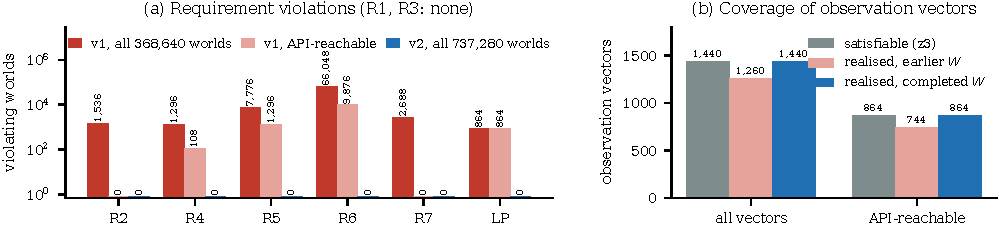
\includegraphics[width=0.9\textwidth]{figs/fig_l1.pdf}
\caption{L1 results. (a) Worlds violating each requirement, for v1 over all worlds, v1 over API-reachable worlds
(the counts of Table~\ref{tab:verdict}), and v2 over all worlds; LP is the employee least-privilege requirement,
with the owner exception of C3. (b) Observation vectors: satisfiable over unbounded
domains (z3), and realised by the world space we used before and after the coverage check.}
\label{fig:l1}
\end{figure*}

\paragraph{Fidelity and drift.} On all 368{,}640 worlds the PDP returned the decision and the deciding rule of
$\mathcal{M}$, without a single indeterminate result (24.5\,s). Our design specification disagrees with it on
18{,}960 worlds. D1 explains all 4{,}032 API-reachable disagreements: the code grants any action in the
assignment, and denies \emph{read} to a subject whose assignment omits it. D2 matters only for division
managers without a division. If the PAP did not forbid those, the D2 exemption would let them past $\Pc$ in
1{,}536 worlds (the R2 bar of Figure~\ref{fig:l1}a), so R2 currently depends on an administrative check.

\begin{theorem}[What v1 gets right]\label{thm:pos}
Under API-reachable states, \chain satisfies R1, R2, R3 and R7 for every number of departments, divisions and
actions.
\end{theorem}
\begin{proof}
Let $\role(u)\neq\mathrm{adm}$. \emph{R1:} its premise is the guard of $P_1$, the first rule that can fire.
\emph{R2:} managers have a division, so $\sameDiv^\circ=\sameDiv$ wherever $\Pc$ applies, and no allow rule
comes before $\Pc$. \emph{R3:} for an employee, $P_4$ needs $a\in\Gasg_t$ and $P_6$ needs $a\in\Gdel_t$.
\emph{R7:} each of the guards of $P_2$, $P_3$, $P_4$ and $P_6$ implies one disjunct. z3 confirms all four with
uninterpreted sorts, including the custom role, in under 10\,ms each.
\end{proof}

\begin{proposition}[The risk rule never changes a decision]\label{prop:inert}
For all $u,o,a$ and all contexts $c,c'$ that differ only in risk signals,
$\pi_d(\decide_{\sigma,t}(u,o,a,c))=\pi_d(\decide_{\sigma,t}(u,o,a,c'))$, where $\pi_d$ projects a result onto
its decision.
\end{proposition}
\begin{proof}
Every allow rule comes before $\Px$, and no guard before $\Px$ mentions $\rho$. So the first applicable rule
among those before $\Px$ is the same in both contexts. If it is an allow rule or an earlier deny rule, both
results agree. Otherwise both evaluations reach $\Px$, and whether $\Px$ or $P_7$ then applies, both deny.
\end{proof}
The \emph{deciding rule} can differ: a custom-role subject without grants is denied by $P_7$ at low risk and by
$\Px$ at high risk. What the proposition rules out is that risk ever turns an allow into a deny.
All 184{,}320 pairs of worlds that differ only in risk get the same decision. Case (c$_2$) of the running
example is one of them. Reading C2 the other way (``risk denies only requests that no allow rule matches'')
does not help: R6 then holds, but only because $P_7$ already implies it, so the rule is dead under either
reading. Our own unit test for $\Px$ passes \emph{because} of this: it checks that a low-risk director is
allowed, which $P_2$ settles first.

\begin{proposition}[A read delegation unlocks writes]\label{prop:unlock}
In some API-reachable state, a non-administrator who holds only a read delegation for an object in another
department is allowed to \emph{write} it.
\end{proposition}
\begin{proof}
$P_1$ only checks $\Gdel\neq\emptyset$, and $P_4$ has no department condition. A division manager $u$ with
$\Gdel_t(u,o)=\{\mathit{read}\}$ and $\mathit{write}\in\Gasg_t(u,o)$ passes $P_1$--$P_3$ and is allowed by $P_4$.
\end{proof}
This is case (b$_2$) of the running example. The object's director may assign anyone, including someone from
another department. We reproduced the state through the API: the write is denied by $P_1$ before the
delegation and allowed by $P_4$ after a read-only delegation is approved (R5, 1{,}296 reachable worlds).

\paragraph{Two more counterexamples.} \emph{R4:} an employee with $\Gdel=\{\mathit{read}\}$ and no assignment is
denied by $P_5$ before $P_6$ is reached, even though the user interface offers employees a ``request access''
button that creates such delegations. Read the other way (C1), the implementation satisfies $P_5$'s
literal description (proved) and the repaired chain does not (z3 counterexample); nothing else depends on C1.
\emph{Least privilege:} an employee whose assignment includes \emph{write} may write (864 worlds), because the PAP
accepts any action list.

\answer{1}{Yes. Criterion G holds for the v1 PDP and the coverage check shows that the bounded world space
realises every satisfiable observation vector, so the L1 check is complete. The PDP matches its model on all
368{,}640 worlds. The chain satisfies R1, R2, R3 and R7, but the risk rule never decides (R6), a read
delegation unlocks writes (R5), delegations are shadowed (R4), and the least-privilege theorem of our design
document is false.}

\subsection{RQ2: The State Level}
\label{sec:l2}

\paragraph{With a cold cache, v1 is right.} On all 420 lifecycle worlds (absent, active, inactive, expired and
not-yet-valid assignments; absent, valid, expired, pending, revoked, rejected and marked-expired delegations) the
PDP's queries agree with $\Gasg_t$ and $\Gdel_t$. Every temporal problem below therefore comes from the cache. Theorem~\ref{thm:stale} (\S\ref{sec:method}) predicts how long each problem lasts.



\begin{figure*}[t]
\centering
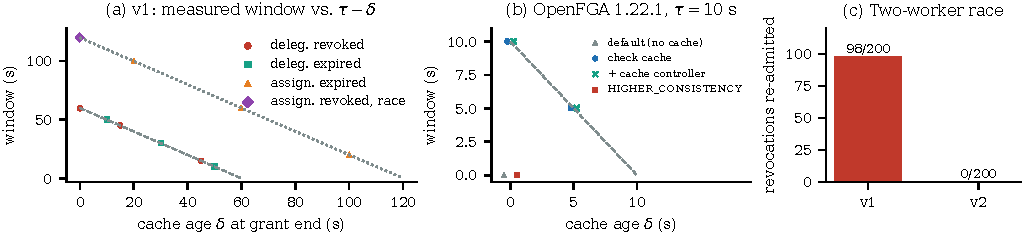
\includegraphics[width=0.92\textwidth]{figs/fig_l2.pdf}
\caption{L2 results. (a) Every v1 staleness trial ($n=10$ per setting) against the prediction $\tau_g-\delta$ of
Theorem~\ref{thm:stale} (dashed: $\tau=60$\,s; dotted: $\tau=120$\,s); the race points use one injected concurrent
decision. (b) OpenFGA, every trial ($n=10$ per setting): with the check cache, with the cache controller added,
with \texttt{HIGHER\_CONSISTENCY}, and in the default configuration; points are offset horizontally for
legibility. (c) Revocations followed by an allow from a re-cached grant under a two-worker server (200 trials
per version).}
\label{fig:l2}
\end{figure*}

\paragraph{Measurements.} Figure~\ref{fig:l2}a and Table~\ref{tab:e2} show ten trials per setting.
Revoking a \emph{delegation} never touches the cache: the windows were 60.1, 45.2, 30.2 and 14.8\,s at
$\delta=0,15,30,45$\,s. Revoking an \emph{assignment} does invalidate, and closed within 0.22\,s with no allowed
decision. \emph{Expiry} is never checked against cached entries, so delegations stayed usable 50.3, 30.2 and
10.3\,s after $t_e$, and assignments 100.3, 60.2 and 20.2\,s after $t_u$. Across all 100 trials, the windows
differ from $\tau_g-\delta$ by between $-0.43$ and $+0.63$\,s, which is about what the 0.25\,s polling interval
and up to 60 concurrent trials should produce (the $\epsilon$ of Theorem~\ref{thm:stale}).

\paragraph{The race.} Assignment revocation invalidates the cache \emph{before} the request transaction commits.
With one decision injected in between, a revoked assignment stayed usable for 120.1 to 120.3\,s ($n=10$).
Without injection, eight decisions racing each revocation in one process left a stale entry in 2 of 60 trials.
We had expected the race to be rare in practice. It is not. Under a server with two workers, \textbf{98 of 200}
revocations (49\,\%; 95\,\% Wilson interval 42--56\,\%) were followed, \emph{after} the revoking request had returned, by an allow decision from a
re-cached grant (Figure~\ref{fig:l2}c). The same harness, run with a single worker during the cost study
(\S\ref{sec:rq5}), counted 174 of 400 (43.5\,\%) in one campaign and 315 of 600 (52.5\,\%) in another: the race
needs concurrent requests, not a second process.
This is adversary class A3: an insider who keeps requesting while an
administrator revokes wins about half the time. Removing a document collaborator behaves like delegation
revocation: no invalidation at all. An open collaboration session is not even consulted. We ran the real
collaboration server against v1, opened a session for a collaborator on a draft, and removed her through the
document API: the API refused her next read at once, but in 10 of 10 trials her session was still open 30\,s
later, with the write permission it had been given at connect (F8).

\begin{table}[t]
\caption{Staleness in v1 ($n=10$ per row): window after the grant ends (median [min, max]) and the largest number
of decisions allowed inside it. Protocol: one decision fills the cache $\delta$ before the grant ends; the window
runs from the return of the revoking request (for expiry, from the end of validity) to the first response of the
decision API that is not an allow, polled with a 0.25\,s pause between requests; the trials of a setting run
concurrently in one server.}
\label{tab:e2}
\footnotesize
\begin{tabular}{@{}l@{\;}r@{\;\;}r@{\;\;}r@{}}
\toprule
Experiment & $\delta$ (s) & window (s) & allows \\
\midrule
Deleg.\ revoked & 0 / 15 & 60.13 [59.59, 60.22] / 45.23 [44.82, 45.44] & 149 / 106 \\
 & 30 / 45 & 30.16 [29.98, 30.28] / 14.84 [14.57, 15.18] & 66 / 27 \\
Deleg.\ expired & 10 / 30 & 50.34 [50.10, 50.63] / 30.24 [30.15, 30.32] & 135 / 82 \\
 & 50 & 10.27 [10.11, 10.50] & 25 \\
Assign.\ expired & 20 / 60 & 100.31 [100.05, 100.44] / 60.24 [60.06, 60.36] & 274 / 156 \\
 & 100 & 20.23 [20.10, 20.40] & 43 \\
Assign.\ revoked & 0 & 0.22 [0.07, 0.22] ($n=5$) & 0 \\
\quad + injected race & 0 & 120.15 [120.09, 120.25] & 453 \\
\bottomrule
\end{tabular}
\end{table}

\paragraph{Mixed views.} We then ran the run of Proposition~\ref{prop:mixed} on the deployment, through the API:
assignment, warming decision, expiry, delegation request and approval, and a write decision 63\,s after the start.
In 10 of 10 trials v1 allowed the write, by $P_4$, and \texttt{/pep/access?action=write} returned
the file, although every committed state of the run denies the request. This allow is not excused by any
staleness tolerance: G1 holds for every $\Delta^\ast$. v2 denied in all 10 trials (by $P_5$), and its file endpoint refused the client-chosen action.

\paragraph{Sessions.} The collaboration server authorizes a WebSocket session once, when it opens. Revoking a
grant has no effect on an open session, so no bound applies on this path at all. Usage control
\cite{park2004ucon} would call this the absence of ongoing authorization.

\answer{2}{With a cold cache, decisions match the stored state. The grant cache keeps revoked or expired grants
usable for $\tau_g-\delta$, as Theorem~\ref{thm:stale} predicts, within 0.63\,s over 100 trials. Invalidating
before the commit lets a race re-admit revoked grants, in 98 of 200 revocations with two workers and in 174 of
400 and 315 of 600 with one; open
collaboration sessions are never re-checked; and because the two grant caches age independently, v1 allowed, in
10 of 10 trials, a write that no committed state allows.}

\subsection{RQ3: The Enforcement Level}
\label{sec:l3}

Reading the code, we found four procedures that decide reads: the \chain PDP, the document service's own
rules, the collaboration server's connect-time check, and a copy of the rules that only decides whether to show
a ``request access'' button; the generated inventory later showed a fifth (F16). Only the decision API and the
file endpoints call the PDP. Table~\ref{tab:l3}
shows the probes that found the failures, and Figure~\ref{fig:l3} the full probe of 57 checks on both versions.

\begin{table*}[t]
\caption{Enforcement probes on the running system, v1 and v2. Ledger cells count durable decision rows per 20
requests; other cells are HTTP status codes. Bold marks a departure from the PDP's decision or from the
requirements.}
\label{tab:l3}
\small
\begin{tabularx}{\textwidth}{@{}p{4.2cm}Xp{1.9cm}p{4.3cm}p{2.3cm}@{}}
\toprule
Probe & Fixture & PDP decision & \sysname v1 & \sysname v2 \\
\midrule
Ledger, \texttt{/pep/access}, \texttt{/preview}, \texttt{/download} & director (allow) / unassigned employee (deny) & allow / deny & allow 20/20; \textbf{deny 0/20 rows}, 0 audit rows & 20/20 and 20/20 \\
Document API \texttt{GET /documents/\{id\}} & published TOP\_SECRET document; employee, \emph{normal} clearance & deny ($\Pc$) & \textbf{200 with full content} (file endpoint on the linked object: 403) & 403 \\
MFA obligation & TOP\_SECRET object; director without MFA & allow ($P_2$) & \texttt{/access} 403; \textbf{\texttt{preview} 200, \texttt{download} 200} & 403 / 403 / 403 \\
Owner bypass & object of another department owned by the requester & deny ($P_1$) & \textbf{\texttt{/access?action=delete} 200; \texttt{download} 200} & 400 / 403 \\
Owner under high risk & own object; $\rho\ge\theta$ (five failed logins, $\theta$ set to 40 for this check) & deny ($\Px$ in $\mathcal{F}$) & \textbf{200} (file and document) & 403 / 403 \\
Change of address & own object and own published document; two failed logins and a new address ($\rho=40$, $\theta$ set to 40) & deny ($\Px$ in $\mathcal{F}$) & \textbf{200} (file and document) & 403 / 403 \\
Deleted object & published document whose object the director deleted; unassigned employee & deny ($P_5$) & \textbf{200 with full content} & 403 \\
Action chosen by the client & assignment \{read\}; \texttt{/pep/download} & deny (download) & \textbf{200 without action parameter} & 403 \\
Revocation authority & unrelated employee of another department & -- & \textbf{revokes a delegation (200) and an assignment (204)} & 403 / 403 \\
Cross-department write & assignment \{read, write\} + read delegation & allow ($P_4$) & \textbf{allowed} (Prop.~\ref{prop:unlock}) & deny \\
Document list \texttt{GET /documents} & published TOP\_SECRET document; employee of the department, \emph{normal} clearance & deny ($\Pc$) & \textbf{listed with full content} & not listed \\
Publishing across departments & approved document; director of another department & deny ($P_1$) & \textbf{200, document published} & 403 \\
\bottomrule
\end{tabularx}
\end{table*}

\begin{figure*}[t]
\centering
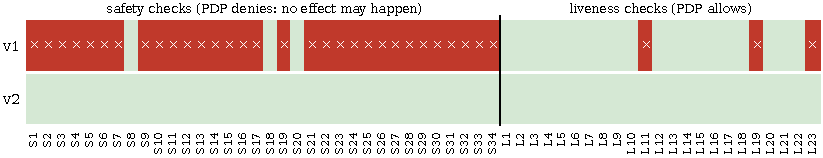
\includegraphics[width=0.92\textwidth]{figs/fig_l3.pdf}
\caption{The L3 probe on v1 and v2: 34 safety checks (S) and 23 liveness checks (L), one run each; a cross marks a
failed check. v1 fails 31 safety checks and three liveness checks. L19 fails because comment resolution always
failed with a server error in v1, L23 only because S33 had already published the document, and L11 only because an unauthorised
director had already revoked the delegation in S15. S19 and S21 use states created through the ORM (a division
manager without a division; a statement-level grant update) that the API of v1 does not produce.}
\label{fig:l3}
\end{figure*}

\paragraph{Lost denials.} The file endpoints write the decision, raise HTTP 403, and let the request
transaction roll back. Every denial disappears together with its audit entry, while the error message tells
the user that the denial ``is permanently logged''. This one embarrassed us most, because denials are precisely
what an investigator needs, and it is what adversary class A6 relies on. The ledger is not append-only either:
deleting a subject cascades into it, and the retention job crashes at run time on a column that does not
exist. Webhook notifications of denials fail too, because they reuse the request's session after it has been
committed.

\paragraph{Paths around the PDP.} The document API lets any employee read any published document of their
department, without an assignment and without the classification test, so it violates R2 and R3, which the PDP
provably satisfies. Unpublished documents fare no better: a collaborator with \emph{normal} clearance reads a
TOP\_SECRET draft, and a division manager reads a TOP\_SECRET department-level document under review. The
collaboration server lets anyone in the department read any document. The owner bypass grants every action
before the PDP runs, attaches no obligations and ignores risk; and since ownership survives a move to another
department, it breaks R1 for owners. Obligations are enforced on one of the three file endpoints, and the
download endpoint evaluates whichever action the client sends.

\paragraph{Administration.} The PDP never reads a policy's status, so the PAP can show a rule as inactive while
it is enforced. The PAP's guard against disabling $P_7$ exists on one of its two update routes, and any
authenticated user can revoke anyone's grants.

\paragraph{Routes we had not listed.} All of the above came from an inventory we had built by reading the code.
We then generated it from the web framework's routing table: 152 API routes, plus four documentation routes and a
metrics endpoint. A static pass over the handlers marks a route as in scope if it can touch an object, a document
or a part of one, return content, or change a grant; 100 are. For each it records which decision procedures the
handler can reach; for v1, six in-scope routes reach none. Four of those are known or deliberate (the revocation
of F14; an access graph documented as visible to everyone; aggregate statistics; document templates); the other
two, comment resolution and signing, are new. Because reaching a procedure does not
mean applying it to the right object, we added two sweeps that need no per-route fixtures. The first sends every
in-scope GET route (48) as an employee of another department and as an unassigned employee of the owning
division, with every text field of the objects marked by kind; the second sends every state-changing route (52)
as those two and as a director and a division manager of another department, against documents in every workflow
state, and compares the database before and after. Together they found four failures (F15--F18 in
Table~\ref{tab:findings}): comment resolution and signing decide nothing; the document list is a fifth decision
procedure, a database query that returns every published document of the department with its content and
ignores $\Pc$, so a TOP\_SECRET document reaches an employee with \emph{normal} clearance; any subject reads any
delegation; and directors and division managers publish, escalate and remove another department's documents and
folders. On v1 the state sweep flags ten routes; on v2 it flags one, because an employee may create a folder in
her own department's space, which no requirement covers. The sweeps also show names and titles of objects the
subject may not read, on six routes of v1 and five of v2. R constrains actions on objects, not their names, so we report these and do not count them as
violations. Nine creation
routes rejected the sweep's minimal bodies (HTTP 422) and one takes a file upload; these ten were not exercised.

\paragraph{Summary of findings.} Table~\ref{tab:findings} collects the eighteen findings of
\S\ref{sec:l1}--\S\ref{sec:l3} and the adversary class each one serves. Fourteen of them lie outside the decision
function.

\begin{table}[t]
\caption{Findings on \sysname v1, by level, adversary class (Table~\ref{tab:adv}) and evidence (P proof; X
exhaustive count; R reproduced on the running system; C code inspection). All are fixed in v2
(\S\ref{sec:rq5}). F15--F18 were found only after the route inventory was generated.}
\label{tab:findings}
\small
\begin{tabularx}{\columnwidth}{@{}l@{\;}l@{\;}l@{\;}X@{\;}l@{}}
\toprule
ID & Lvl & Cl. & Finding & Ev. \\
\midrule
F1 & L1 & A1 & Risk rule $\Px$ never decides (Prop.~\ref{prop:inert}) & P,X \\
F2 & L1 & A1 & $P_5$ shadows employee delegations (R4) & P,X \\
F3 & L1 & A1 & Read delegation unlocks cross-department writes & P,X,R \\
F4 & L1 & A1 & Spec drift D1--D3; least-privilege theorem false & P,X \\
F5 & L2 & A2 & Delegation revocation and collaborator removal never invalidate & R,C \\
F6 & L2 & A2 & Validity bounds ignored for cached grants & R \\
F7 & L2 & A3 & Invalidation before commit re-admits revoked grants (44--53\,\% of trials) & R \\
F8 & L2 & A2 & Collaboration sessions authorized only at connect & R,C \\
F9 & L2 & A2 & Mixed cached views allow what no committed state allows & P,R \\
F10 & L3 & A6 & Denials rolled back; ledger not append-only; retention job crashes & R,C \\
F11 & L3 & A4 & Document API and collaboration server bypass the PDP & R,C \\
F12 & L3 & A5 & Owner bypass grants every action, ignores risk, survives a change of department & R \\
F13 & L3 & A4 & Obligations on one endpoint only; client chooses the action & R \\
F14 & L3 & A7 & PAP status ignored by the PDP; revocation needs no authority & R,C \\
F15 & L3 & A4 & Comment resolution and signing call no decision procedure & R,C \\
F16 & L3 & A4 & Document list decides on its own: content of every published document, no $\Pc$ & R \\
F17 & L3 & A4 & Any subject reads any delegation & R \\
F18 & L3 & A4 & Publishing, escalation and folder removal across departments & R \\
\bottomrule
\end{tabularx}
\end{table}

\answer{3}{Five procedures decide reads, and only the decision API and the file endpoints ask the PDP. The
document API, the document list and the collaboration server bypass it, the owner rule skips it, obligations
are enforced on one of three file endpoints, the client chooses the action, denials are never recorded, anyone
can revoke grants, and several routes decide nothing or ignore the department. Fourteen of the eighteen findings
lie outside the decision function, and four of them appeared only once the route inventory was generated from
the routing table instead of read from the code.}

\subsection{RQ4: Which Oracle Sees Which Fault?}
\label{sec:adequacy}

Our repository has 140 tests: 22 unit, 42 ``conformance'' and 76 integration tests. As committed, 59 of the 76
integration tests fail when run together, because of a hard-coded login limit and a CSRF header that the tests
predate. We lifted both with an external pytest plugin, without changing the application, and then all 138
non-skipped tests of v1 pass (2 are skipped). Coverage is 95\,\% for the PDP, but only 25\,\% for the PEP and 28\,\% for the delegation
workflow. The coverage numbers turned out to predict the mutation results quite well.

\paragraph{Decision logic.} We generated 96 mutants of the v1 PDP. Of these, 13 are equivalent on valid inputs,
3 differ only at the instant a validity bound is reached, and 1 needs inconsistent administrator flags, which
leaves 79. The 3 boundary mutants are not harmless: a frozen-clock oracle that sets a grant's bound equal to the
clock kills all three, and two of them allow a request at the very instant its grant ends.
Figure~\ref{fig:mut}a shows how many each oracle kills. The 11 that escape the L1 oracle all change the database
queries on the cache-miss path, and the L2 cold-cache oracle kills every one of them. Of the 7 that escape our
whole repository suite, 4 are state-level mutants that only E1b detects: they honour assignments that are not yet
valid, delegations held by other subjects, delegations for other objects, and delegations that were never
approved.

\paragraph{Enforcement and cache code.} We then mutated the code we had written for v2: the single PEP gate, the
document-read decision, both revocation handlers, the versioned cache, the post-commit invalidation hooks, and the
middleware that passes the client address to the document route. The same operators as above give 159 mutants of
the final v2; we drop the 2 that mutate the switch used only by the cost ablation, which leaves 157 (the set
differs from earlier versions because the gate and document code changed). The repository suite kills 21 of them
(13.4\,\%) and the 57-check L3 probe kills 116 (73.9\,\%); together they kill 118 (75.2\,\%), and only 2 are
killed by the repository suite alone (Figure~\ref{fig:mut}b). The probe grew with the analysis. A first version
with 11 safety and 6 liveness checks killed 72 of the 158 mutants of an earlier v2; the survivors that could grant
access led to new checks, and the 29-check version killed 105 of those 158. A 38-check version missed a mutant
that drops the address-change term of $\rho$, because no check changed the client address; the checks S24--S25
now do, and kill it. The 39 survivors of the final run are shown in Figure~\ref{fig:mut}c. We inspected each one
by hand:
\begin{itemize}
\item 11 only stop the grant cache from being read or written, so every decision falls back to the database;
\item 7 are equivalent on the attribute domain (for example, no clearance has rank below~1, so comparing with 0, 1
or $-1$ in the classification barrier gives the same result);
\item 5 scale a cache lifetime by $\pm0.1\,\%$ or move a cut-off by 1\,ms;
\item 3 change only decision metadata, such as the measured latency;
\item 3 change the notice sent after a revocation;
\item 2 are masked by a redundant defence: the cache entry's lifetime already ends with the grant, so the expiry
check at read time never fires;
\item 2 make the cache return a malformed value after a Redis error, which the PDP rejects with a server error,
so the request fails closed;
\item 2 change the decision only for a published document with no linked object at all, a state that no route
creates (publishing always links an object, and objects are only deactivated, never removed);
\item 1 bumps the global generation on every bulk write, which only causes extra cache misses.
\end{itemize}
These 36 survivors cannot change a decision, an effect or a record in a state the API can reach. The other three
can. The first makes the document route's risk check strict ($>$ instead of $\geq$), so a request whose score is
exactly $\theta$ is no longer denied there; for a published document the PDP's own $\Px$ still denies it, but for
an unpublished one the workflow rules can then allow it. The probe's risk fixtures reach $\theta$ only on published documents, where the PDP's own check also denies.
The second flips the department test of the owner exemption from the barrier, so an owner whose clearance is
below her own draft's sensitivity can no longer read it; nothing is granted, but access is lost. The third gives
internal calls from the collaboration server that server's address instead of \texttt{unknown}, so the
address-change term can refuse a collaborator's session; again it can only deny. We then ran the bounded
document check E1c (\S\ref{sec:rq5}) against the document survivors. It kills the first two (the first through
97{,}524 R6 violations at $\rho=\theta$, all on unpublished documents, the second through 11{,}016 disagreements
with $\mathcal{M}_{\mathrm{doc}}$) and both unreachable-state mutants (11{,}520 violations of R1--R3 each), and agrees on every world with the three equivalent ones.
Nothing we have kills the third. The lesson is the one the earlier versions taught: a probe checks only the
inputs its fixtures vary, and a bounded check of the same procedure covers the values in between.

\paragraph{Held-out operators.} Because the probe grew while we studied survivors of the operators above, its
score on them may flatter it. We therefore froze the 57-check probe and applied three operators we had not used
while building it, to the same functions: statement deletion, turning a \texttt{raise} into a silent return, and
swapping the first two arguments of a call. This gives 111 mutants; 2 fall inside the ablation switch, which
leaves 109. The probe kills 76 (69.7\,\%), close to its 73.9\,\% on the original operators, and the repository
suite kills 34 (31.2\,\%), every one of which the probe also kills. Of the 33 survivors, 30 cannot change a
decision, an effect or a record: 7 bypass the cache, 6 are equivalent (for example, a flush that the commit at
the end of the request repeats), 6 are masked by a redundant defence (each grant entry is keyed by both the
subject's and the object's counter, so dropping either increment is harmless), 6 only change an error response,
3 change metadata that no rule reads, and 2 change the revocation notice. Three can change a record, and none can
grant access: two drop the audit row written when a delegation or an assignment is revoked (the revocation still
takes effect), and one lets an authorised revoker revoke a delegation that was never approved. The probe counts
the decision and audit rows of access requests, not of administrative changes, so both gaps are again inputs it
does not vary.

\begin{figure*}[t]
\centering
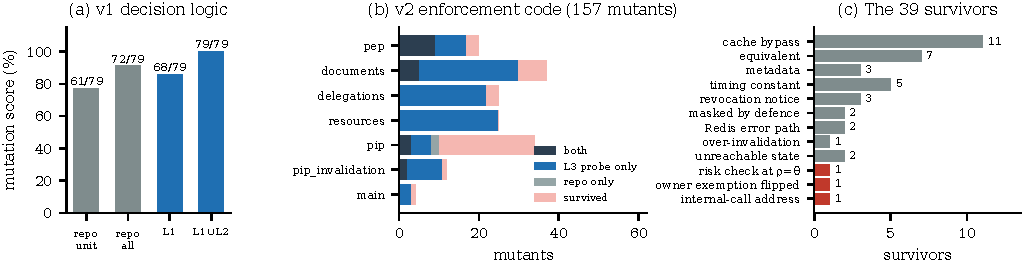
\includegraphics[width=0.92\textwidth]{figs/fig_mut.pdf}
\caption{Mutation analysis. (a) v1 decision logic: share of the 79 non-equivalent PDP mutants killed by each
oracle. (b) v2 enforcement and cache code: mutants per file by the oracle that kills them (repository suite,
L3 probe, both) or surviving. (c) The survivors of (b), by class; grey classes cannot change a decision in a
state the API can reach, red ones can.}
\label{fig:mut}
\end{figure*}

\begin{table}[t]
\caption{Mutation scores per oracle. Top: v1 PDP decision logic (79 non-equivalent mutants). Bottom:
enforcement and cache code of v2, with the original and with held-out operators.}
\label{tab:mut}
\small
\begin{tabular}{@{}lrr@{}}
\toprule
Oracle & killed & score \\
\midrule
Repository unit + conformance suites & 61 / 79 & 77.2\,\% \\
Repository, all 140 tests & 72 / 79 & 91.1\,\% \\
L1 differential oracle (E1) & 68 / 79 & 86.1\,\% \\
L1 $\cup$ L2 (E1, E1b) & 79 / 79 & 100\,\% \\
\midrule
Repository suite on v2 enforcement code & 21 / 157 & 13.4\,\% \\
L3 probe, first version (11 + 6 checks)$^{*}$ & 72 / 158 & 45.6\,\% \\
L3 probe, 29 checks$^{*}$ & 105 / 158 & 66.5\,\% \\
L3 probe, final (34 + 23 checks) & 116 / 157 & 73.9\,\% \\
Repository suite $\cup$ final L3 probe & 118 / 157 & 75.2\,\% \\
Held-out operators: repository suite & 34 / 109 & 31.2\,\% \\
Held-out operators: frozen L3 probe & 76 / 109 & 69.7\,\% \\
\midrule
\multicolumn{3}{@{}p{0.95\columnwidth}@{}}{\footnotesize $^{*}$On an earlier v2 (158 mutants). Of the 39 survivors
of the final run, 36 cannot change a decision, effect or record in a reachable state; E1c kills two of the other
three (Fig.~\ref{fig:mut}c).} \\
\bottomrule
\end{tabular}
\end{table}

\answer{4}{Our repository's tests catch faults in the decision logic (72 of 79 mutants) but hardly any in the
enforcement and cache code (21 of 157). The level oracles catch both: L1 and L2 together kill all 79 decision
mutants, and the L3 probe kills 116 of the 157 enforcement mutants. Of the 39 survivors, three can change a
decision in a reachable state; a bounded check of the document procedure kills two of them. On operators held
out while it was built, the frozen probe scores about the same (76 of 109), and no survivor can grant access.
Each survivor that mattered pointed at an input our fixtures did not vary, not at a fault in v2.}

\subsection{RQ5: Repair, Cost and Comparison}
\label{sec:rq5}

\subsubsection{Repairing \sysname}

\paragraph{Design rules.} The findings suggest six rules.
\textbf{DR1}: put risk denies before every allow rule, or use deny-overrides, and lint for deny-after-permit
redundancy.
\textbf{DR2}: test grants as $a\in G$, keep the scope condition in every allow rule, and let a delegation
actually reach its allow rule.
\textbf{DR3}: make cached grants validity-aware ($\mathit{TTL}=\min(\tau,t_{\mathrm{end}}-t)$) and versioned, and
invalidate \emph{after} the commit, much as Zanzibar uses consistency tokens \cite{pang2019zanzibar}.
\textbf{DR4}: send every protected read through one decision procedure, and let the endpoint, not the client,
choose the action.
\textbf{DR5}: write decisions in their own transaction.
\textbf{DR6}: test each property at the level where it lives.

\paragraph{The repaired chain.} $\mathcal{F}$ moves $\Px$ to just after the administrator rule, adds $\sameDept$ to
$P_4$, puts $P_6$ before $P_5$ (which then denies every employee who holds no grant for the action), and uses
$\sameDiv$. It also makes the owner rule a rule of the chain: $\Po$, with guard $\ow(u,o,a)$, follows $P_3$, and
$\Pc$ exempts it as it exempts $P_2$ and $P_3$ (C3). In v1 this rule was a constant outside the PDP
(\S\ref{sec:system}). Finally, $P_4$ grants read only, whatever else the assignment lists, which removes drift D1
(C4). z3 proves every requirement, R1--R7 and LP, for $\mathcal{F}$ over unbounded domains
(Table~\ref{tab:verdict}). LP holds with the owner exception: an owner needs no assignment to open her own
object.

\paragraph{\sysname v2.} We implemented DR1--DR5 as v2 (15 files, $+$579/$-$289 lines, kept in a separate
history whose first commit is v1). Most of it is straightforward. The cache is not, so Algorithm~\ref{alg:cache} and
Figure~\ref{fig:cache} describe it in detail. Every cached grant is keyed by three generation counters, one global, one per
subject and one per object. A cache fill uses the counters it read \emph{before} querying the database. An
SQLAlchemy \texttt{after\_commit} hook bumps the counters for every ORM or bulk change to a grant, so no endpoint
has to remember to invalidate. Entries also carry the grant's end of validity. Beyond the cache, v2 changes
eight things. One gate serves all file endpoints and decides every request with the PDP, owners included.
Document reads are decided by the PDP on the linked object, with the same request context as the gate, and
every route that lists documents or reads or changes their parts (comments, signatures, delegations shown with
them) applies the same decision, while workflow routes act only within the actor's department. An assignment
grants read only.
Decision and audit rows are written in their own transactions. Revocation requires authority. The PAP refuses to
show built-in rules as inactive. The collaboration server re-checks open sessions every 5\,s. Figure~\ref{fig:v2} shows the
resulting request paths next to those of v1 (Figure~\ref{fig:system}).

Our first version of v2 still had a hole, and we only noticed it while drawing that figure. The design of
\sysname lets an object's owner act on it. The first v2 kept that rule in the gate, confined to the owner's
department and with obligations attached, but still \emph{before} the PDP, and so before $\Px$: a high-risk owner
was allowed where $\mathcal{F}$ denies. DR1 held in the PDP and failed at the gate. None of our probes had a
high-risk owner. Our second version evaluated $\Px$ before the owner rule, in the gate and in the document
procedure, and the probe gained two checks (S22, S23). That closed the hole but kept a second decision procedure
for owners, against DR4, and the document procedure had no request address, so its $\Px$ ignored a change of
address. The current v2 removes both: the owner rule is $\Po$ inside the PDP, the gate and the document procedure
only call the PDP, and both pass the request address to it. Three further checks (S24--S26) cover this, and two
liveness checks (L16, L17) keep it from denying too much.

Another hole was in code we had never run. Our fix for F8 adds a loop to the collaboration server that
re-checks every open session every 5\,s. When we first ran the server, for this paper's final measurements, the
loop re-checked nothing: it looked for the open sessions under a property that the version of the
collaboration library we depend on does not have, so it found none, and a removed collaborator kept her session
(0 of 5 trials closed within 30\,s). After a one-line fix, the server closed the session in 10 of 10 trials,
1.9--4.8\,s after the removal, within the bound of the 5\,s period plus one decision. Our probes had exercised
every request path we had listed in the backend, but not the collaboration server, which is a process of its own.

The list itself was the next weakness. Until then, our route inventory came from reading the code. We then
generated it from the web framework's routing table (\S\ref{sec:l3}), probed what it showed, and swept every
route in scope with subjects who must be refused. This found four more holes, all inherited from v1: comment
resolution and signing decided nothing (F15); the document list decided with a query of its own that showed
every published document of the department, content included, and ignored the classification barrier (F16);
any subject could read any delegation (F17); and a director or division manager of one department could
publish, escalate or remove another department's documents and folders (F18). Each fix makes the route apply
the decision its single-object counterpart applies. Seven safety checks (S28--S34) and five liveness checks
(L19--L23) cover them and the read-only assignments; the first liveness check also showed that comment
resolution had always failed with a server error, which we fixed too.

\begin{figure}[t]
\centering
\begin{tikzpicture}[
  font=\scriptsize, node distance=2mm,
  box/.style={draw, rounded corners=1.5pt, align=center, inner sep=1.5pt, minimum height=5mm},
  pep/.style={box, fill=blue!6, text width=17mm},
  dp/.style={box, fill=green!8, text width=20mm},
  st/.style={box, fill=orange!10, text width=14mm},
  arr/.style={-{Stealth[length=1.5mm]}, semithick}]
  \node[pep] (b1) {\texttt{/access/decide}};
  \node[pep, below=of b1] (b2) {\texttt{/pep/access}, \texttt{/preview}, \texttt{/download}};
  \node[pep, below=of b2] (b3) {\texttt{/documents},\\\texttt{/documents/\{id\}}\\and its parts};
  \node[pep, below=of b3] (b4) {collab.\ WebSocket\\(connect, every 5\,s)};
  \node[dp, right=4mm of b2] (gate) {one gate: PDP for every request, owners included; action from endpoint; obligations};
  \node[dp, right=4mm of b3, yshift=-5mm] (doc) {document read: $\Px$ with request address; published $\to$ PDP; draft $\to$ $\Pc$ barrier};
  \node[dp, text width=11mm, right=4mm of gate] (pdp) {PDP\\$=\mathcal{F}$};
  \node[st, right=4mm of pdp, yshift=7mm] (cache) {versioned grant cache};
  \node[st, below=4mm of cache] (pg) {PostgreSQL};
  \node[st, below=4mm of pg] (log) {ledger (own transaction)};
  \draw[arr] (b1.east) -| (pdp.north);
  \draw[arr] (b2) -- (gate); \draw[arr] (gate) -- (pdp);
  \draw[arr] (b3.east) -- (doc.west); \draw[arr] (b4.east) -- (doc.west);
  \draw[arr] (doc.east) -| (pdp.south);
  \draw[arr] (pdp.east) -- (cache.west); \draw[arr] ([xshift=-2mm]cache.south) -- node[left]{miss} ([xshift=-2mm]pg.north);
  \draw[arr, dotted] ([xshift=2mm]pg.north) -- node[right]{bump} ([xshift=2mm]cache.south);
  \draw[arr, dashed] (pdp.south east) -- (log.west);
\end{tikzpicture}
\caption{\sysname~v2: every protected read passes $\Px$ first and is then decided by the PDP (which contains the
owner rule $\Po$) or, for unpublished documents, by the clearance barrier of $\Pc$ followed by the document
rules. Decisions are recorded in their own transaction, and committed grant changes bump the cache
generations.}
\label{fig:v2}
\end{figure}

\begin{algorithm}[t]
\caption{Versioned, validity-aware grant cache (v2)}
\label{alg:cache}
\SetKwFunction{Get}{Lookup}\SetKwFunction{Fill}{Fill}\SetKwFunction{Bump}{OnCommit}
\SetKwProg{Fn}{function}{:}{}
\Fn{\Get{$u,o,g$}}{
  $\vec{n}\gets(\mathit{gen}_\ast,\mathit{gen}_u,\mathit{gen}_o)$ \tcp*{one atomic read}
  remember $\vec{n}$ for this request\;
  $e\gets\mathit{cache}[g,u,o,\vec{n}]$\;
  \lIf{$e\neq\bot\wedge \mathit{now}<e.\mathit{exp}$}{\Return $e.\mathit{actions}$}
  \Return miss\;
}
\Fn{\Fill{$u,o,g,B,t_{\mathrm{end}}$}}{
  $\vec{n}\gets$ the generations remembered \emph{before} the database read\;
  $\mathit{ttl}\gets\min(\tau_g,\,t_{\mathrm{end}}-\mathit{now})$\;
  \lIf{$\mathit{ttl}>0$}{$\mathit{cache}[g,u,o,\vec{n}]\gets(B,t_{\mathrm{end}})$ with lifetime $\mathit{ttl}$}
}
\Fn{\Bump{$\mathit{tx}$}}{
  \ForEach{grant row $(u,o)$ inserted, updated or deleted in $\mathit{tx}$}{increment $\mathit{gen}_u$, $\mathit{gen}_o$}
  \lIf{$\mathit{tx}$ ran a bulk statement on a grant table}{increment $\mathit{gen}_\ast$}
}
\end{algorithm}

\begin{figure}[t]
\centering
\begin{tikzpicture}[font=\scriptsize, >={Stealth[length=1.4mm]}]
  \draw[->] (0,0) -- (6.9,0) node[right]{$t$};
  \node[anchor=east] at (0,0.8) {revoke};
  \node[anchor=east] at (0,-0.8) {decision};
  \draw[thick, blue!60] (0.2,0.8) -- (3.8,0.8) node[midway, above]{revoking transaction};
  \draw[fill=blue!60] (3.8,0.8) circle (1.4pt) node[below=1pt]{commit};
  \draw[fill=red!70] (5.0,0.8) circle (1.4pt) node[above=1pt]{$\mathit{gen}_u\gets k{+}1$};
  \draw[thick, teal] (1.4,-0.8) -- (6.3,-0.8);
  \draw[fill=teal] (1.4,-0.8) circle (1.4pt) node[below=1pt]{read gens: $k$};
  \draw[fill=teal] (3.1,-0.8) circle (1.4pt) node[below=1pt]{DB read (old state)};
  \draw[fill=teal] (6.3,-0.8) circle (1.4pt) node[below=1pt]{fill under $k$};
  \draw[dashed, gray] (5.0,0.65) -- (5.0,-1.15);
  \node[align=center, text width=64mm] at (3.4,-1.6) {every lookup after the bump uses generation $k{+}1$, so the stale fill is never served};
\end{tikzpicture}
\caption{Why the v2 cache closes the race: a fill that read the database before the commit is stored under the
old generation, which no lookup after the commit can reach.}
\label{fig:cache}
\end{figure}

The cache earns a small theorem of its own, in the safe direction: whatever it reports as granted was granted
recently.

\begin{proposition}[Freshness of the v2 cache]\label{prop:fresh}
Assume (i) every committed transaction that changes a grant of $(u,o)$ increments $\mathit{gen}_u$ and
$\mathit{gen}_o$, or $\mathit{gen}_\ast$ for a bulk statement, within $\epsilon_b$ of its commit; (ii)
\textsc{Fill} stores the action set read from committed state under generations observed before that read;
(iii) no entry is served at or after its grant's end of validity; (iv) \textsc{Lookup} reads the generation vector
and the entry in one atomic step, which is its linearization point $t$ in the sense of
\cite{herlihy1990linearizability}; and (v) counters never decrease. If \textsc{Lookup} at time $t$ returns $B$ for
$(u,o,g)$, then $B=G^g_{t'}(u,o)$ for some $t'\in[t-\epsilon_b,t]$, unless the grant became valid at a future
start time without any commit, which can only make the cache deny.
\end{proposition}
\begin{proof}
Let the entry have been filled from a read of $\sigma_{t_r}$ under generations $\vec{n}$ observed at
$t_n\le t_r$; so $B=G^g_{t_r}(u,o)$, possibly up to grants that ended after $t_r$, which (iii) excludes. If
$t_r\ge t-\epsilon_b$, take $t'=t_r$. Otherwise suppose some commit at $t_c\in(t_r,t-\epsilon_b]$ changed a grant
of $(u,o)$. By (i) a generation in $\vec{n}$ was incremented by $t_c+\epsilon_b\le t$. Counters only grow, so the
lookup at $t$ read a vector different from $\vec{n}$ and could not have found the entry, a contradiction. Hence
no grant of $(u,o)$ changed by commit in $(t_r,t-\epsilon_b]$, and with (iii) $B=G^g_{t-\epsilon_b}(u,o)$.
\end{proof}

In the code, (i) holds with $\epsilon_b$ the time between the database commit and the Redis increments in the
same process; (ii) holds because the generations read at the miss are kept in the request context and reused
by the fill; (iii) is enforced twice, by the entry's lifetime and by an explicit check; (iv) holds because one Redis
script reads the counters and the entry; and (v) holds because counters and entries live in the same Redis, so a
restart or flush removes both. Assumption (i) is conditional: if the increments fail, for instance because Redis
is unreachable, the hook logs the failure and only Theorem~\ref{thm:stale} applies, bounding the window by
$\tau_g$. A crash between commit and increment has the same effect.

We measured both cases on the running server. Under a load of 16 clients sending file requests, we created and
revoked an assignment 200 times, with one and with two server workers, and timed the hook in the server process.
Over the 400 commits of each setting, $\epsilon_b$ had a median of 0.79 and 0.70\,ms, a 99th percentile of 3.7 and
3.0\,ms, and a maximum of 4.8 and 4.4\,ms; in all 400 revocations the counters had moved before the revocation's
response was sent, and the next request was denied. We then made the hook's connection to Redis fail during the
revocation, while the cache itself stayed up, in five trials each with a refused connection and with a timeout.
In all ten, the increment was lost and the revoked grant kept working for 118--120\,s, that is, until the
cached entry's lifetime of $\tau_{\mathrm{asg}}=120$\,s ran out, as Theorem~\ref{thm:stale} predicts. The timeout
also showed a cost we had not expected: the hook uses a synchronous Redis client, so the 2\,s timeout blocks the
server's event loop, and an unrelated request sent meanwhile took 1.8\,s instead of 12--21\,ms.

Both grant kinds use the same counters, so a commit on either invalidates both entries of the pair, and the two
grant sets of a decision come from states at most $\epsilon_b$ apart. That is still a view, not a snapshot, but
$\mathcal{F}$ satisfies the premise of Proposition~\ref{prop:witness}. Hence every v2 allow is justified by a
committed state at most $\epsilon_b$ old, provided the attributes of $u$ and $o$ (read from the database at decision
time) did not change in that interval: v2 is L2$^+_{\epsilon_b}$ under this proviso, and with the gate it meets the
premise of Theorem~\ref{thm:compose} with $\Delta=\epsilon_b$.

\smallskip\noindent\fbox{\parbox{\dimexpr\columnwidth-2\fboxsep-2\fboxrule\relax}{\small
\textbf{What the end-to-end guarantee for v2 assumes.} Theorem~\ref{thm:compose} gives, for v2, that every effect is
justified by a committed state at most $\epsilon_b+d$ old, and every decision is recorded, if:
\begin{enumerate}[leftmargin=*,nosep]
\item runs are well-formed (W1--W3, Def.~\ref{def:runs}), and an effect follows its decision within $d$;
\item every committed grant change increments its counters within $\epsilon_b$ (measured: at most 4.8\,ms under load);
\item the subject's and object's attributes do not change between the cache fill and the decision (they are read
from PostgreSQL at each decision, at the default isolation level, \texttt{READ COMMITTED});
\item the trusted base of \S\ref{sec:threat} (database, cache, administrators, deployed code) is not compromised;
\item every path to a protected object is in the L3 inventory and its checks pass.
\end{enumerate}
If (2) fails because Redis is unreachable at commit, only the TTL bound $\Delta=\tau$ of Theorem~\ref{thm:stale}
holds (measured: 120\,s for assignments). The guarantee is never one of current-state authorization: an effect
may follow a revocation by up to $\Delta+d$.}}

\paragraph{Does it work?} The v2 PDP equals $\mathcal{F}$ on all 737{,}280 worlds (the 368{,}640 of v1, once
with and once without ownership), violates none of the requirements, LP included (Figure~\ref{fig:l1}a), and
still satisfies criterion G (96 occurrences; the self-test still flags all ten seeded violations). Its observation vector gains two atoms, $[\mathsf{own}(o)=u]$ and $[a=\mathit{download}]$; with them, the
coverage query finds 4{,}320 satisfiable vectors, all realised by the world space, so Theorem~\ref{thm:complete}
applies to v2 as well. With a cold cache, its queries agree with $\Gasg_t$ and $\Gdel_t$ on all 420 lifecycle
worlds, as v1's do. All 57 checks of the L3 probe pass on v2, while v1 fails 31 of the 34 safety checks
(Figure~\ref{fig:l3}), and denials leave 20 of 20 rows on every endpoint. The version of v2 before this paper's last
round of fixes fails all seven new safety checks (S28--S34) and two liveness checks (L19, with a server error,
and L23, because S33 had already published its document), which is how we confirmed that the checks see the holes
they were written for.

The document procedure is not the PDP for unpublished documents, so we gave it an L1 check of its own. We
transcribed it as a reference $\mathcal{M}_{\mathrm{doc}}$ and drove the real procedure, with only its data
sources stubbed as in E1, over 604{,}800 worlds: every role, division and department relation, workflow status,
clearance and sensitivity, ownership, collaboration, linked object (none, active, deleted), grant on that object,
and risk. We checked agreement with $\mathcal{M}_{\mathrm{doc}}$, R1, R2, R3 and R6 (for documents, R3 also accepts
a collaboration invitation on an unpublished document, the guide's mechanism for co-editing drafts), and that a
published document is decided as $\mathcal{F}$ decides its object. The check found a third hole in v2. Deleting a
published document's object (an ordinary soft delete through the API) left the document published, and its reads
fell through to the workflow rules: any employee of the department could read it without a grant (R3), a subject
who had moved could read it with an old assignment (R1), and an owner who had moved escaped the clearance barrier
(R2). The three requirements failed in 384, 1{,}344 and 480 worlds, and 2{,}253 worlds with a deleted object were
decided differently from $\mathcal{F}$. (R3 also failed in 216 worlds of a published document with no object at
all, which the API cannot produce.) The current v2 lets the linked object decide through the PDP whether or not it is
active, refuses a published document without one, and confines the owner's exemption from the barrier to her
department; the check then reports no violation, and the probe has a check for it (S27). All staleness windows shrink to the
resolution of the harness: 0.03--0.05\,s after delegation revocation, 0.02--0.14\,s after expiry, 0.02\,s with the
injected race, and no stale allow in 200 two-worker races (Figure~\ref{fig:l2}c; upper 95\,\% bound 1.9\,\%) or,
on the final v2, in 600 one-worker races (0.6\,\%); the cache and revocation code has not changed since these staleness runs. Of our 140 tests, on v2
137 pass, 2 are skipped (as on v1) and 1 fails. The one that fails asserts that $P_7$, not $P_5$, denies a request
that both rules deny; in $\mathcal{F}$, $P_5$ denies every employee who holds no grant for the action, so it
decides first.

\subsubsection{Cost}

We measured v1 and the final v2 with 16 closed-loop clients on one server worker, three interleaved runs per
version, and 3{,}000 requests per workload and run (Figure~\ref{fig:cost}). On this machine, runs of the same
version differed by up to 42\,\% in their median, so we report a difference only where every run of one version
lies on the same side of every run of the other. Three differences pass that test. Denied file requests, which v2 records in their own transaction, are
32\,\% slower (median 104 to 136\,ms); document reads, which now pay for a full PDP decision and an unindexed
lookup of the linked object, are 47\,\% slower (110 to 162\,ms); and assignment creation is 35\,\% faster (169 to
110\,ms), probably because one counter increment replaces two scans of the cache's key space. For
decisions and allowed file requests, the pooled medians of v2 are 2--9\,\% higher, but the runs overlap, so we
cannot tell them apart from the noise. The 99th percentile of document reads rises from 224 to 326\,ms, and their
throughput falls by 34\,\%; no request failed with a server error in either version. The revocation race,
repeated within these runs, re-admitted a revoked grant in 315 of 600 trials on v1 (52.5\,\%; 95\,\% Wilson
interval 48.5--56.5\,\%) and in none of 600 on v2 (upper bound 0.6\,\%). An earlier measurement with two runs per
version, on a quieter machine and before the last changes to the gate and the document route, gave higher ratios
for decisions (16--25\,\%) and documents (69\,\%); we do not know how much of that gap is the code and how much the
machine. We also ran two workers on an earlier v2. There, medians of the \emph{same} version differed by up to
67\,\% between runs; we suspect an uneven split of the client connections between the two workers, did not verify
it, and draw no conclusion from those runs. Where the cost matters, the obvious next steps are an index on the
document link and batching the decision log; we have not done either.

\begin{figure}[t]
\centering
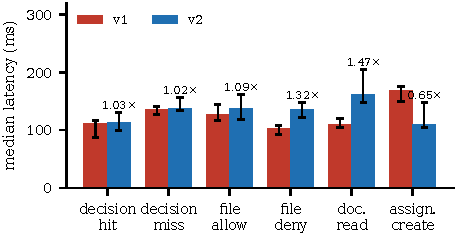
\includegraphics[width=\columnwidth]{figs/fig_cost.pdf}
\caption{Median latency of v1 and the final v2 on one server worker, 16 clients, three runs per version
($n=9{,}000$ per bar). Error bars span the three per-run medians; labels give the ratio v2/v1 of the pooled
medians. Only denied file requests, document reads and assignment creation differ by more than the spread between
runs.}
\label{fig:cost}
\end{figure}

\subsubsection{\chain in Cedar}

A first-applicable chain compiles exactly into Cedar's forbid-overrides semantics. Rule $i$ becomes a
\texttt{permit} when $e_i=\allowv$ and a \texttt{forbid} when $e_i=\denyv$, with the condition
\[
\gamma_i\wedge\textstyle\bigwedge_{j<i,\;e_j\neq e_i}\neg\gamma_j .
\]
A permit fires only if no earlier deny guard holds, and a forbid only if no earlier allow guard holds, so the
first applicable rule decides and no forbid can override it. Cedar's actions are fixed by its schema, so grant
membership expands per action. The compiled policies for $\mathcal{M}$ (36) and $\mathcal{F}$ (40) pass Cedar's
validator, and Cedar's authorizer agrees with our reference on every request: 368{,}640 for $\mathcal{M}$, and
737{,}280 for $\mathcal{F}$, whose owner rule doubles the request space (the requester owns the object or not).
The translation also makes F1 easy to see: in $\mathcal{M}$, the $\Px$ forbid is guarded by the negation of every
allow scope, and deleting it changes nothing. A hand-written 12-policy version of $\mathcal{F}$, with plain
\texttt{forbid} rules for $\Px$, $P_1$ and $\Pc$ and the owner exemption as an \texttt{unless} clause, agrees on
all 737{,}280 requests as well. Under forbid-overrides, DR1 holds by construction.

\subsubsection{\sysname Among Other Authorization Systems}
\label{sec:compare}

We wanted to know whether what we found is specific to our code, and how our design choices compare. We
therefore applied parts of the method, without modifying the systems, to three independent ones. This is a
preliminary transfer: we ran sampled L1 checks, targeted L2 experiments and a few L3 probes, but established
neither criterion G nor coverage nor a route inventory for their code. The systems are:
\begin{itemize}
\item OpenFGA 1.22.1 \cite{openfga}, an open implementation of Zanzibar's relationship model, run from its
release binary;
\item Cedar's TinyTodo sample application \cite{cedarexamples}, built on a verified authorizer;
\item the Backstage RBAC plugin 8.1.6 \cite{backstagerbac}, which keeps policies in a database and takes groups
from a software catalog.
\end{itemize} Zanzibar
itself is not available to run, so we compare with it from its paper \cite{pang2019zanzibar}.
Table~\ref{tab:compare} puts the six side by side; every cell is either measured by us, cited, or marked as not
evaluated.

\begin{table*}[t]
\caption{\sysname compared with other authorization systems. M: measured by us on an unmodified system; C: from
the cited source; n.e.: not evaluated. Bold marks a failure found by our method.}
\label{tab:compare}
\footnotesize
\begin{tabularx}{\textwidth}{@{}l@{\;\;}X@{\;\;}X@{\;\;}X@{\;\;}X@{\;\;}X@{\;\;}X@{}}
\toprule
 & \sysname v1 (M) & \sysname v2 (M) & Zanzibar \cite{pang2019zanzibar} (C) & OpenFGA 1.22.1 (M) & Cedar, TinyTodo (M) & Backstage RBAC 8.1.6 (M) \\
\midrule
Policy model & ABAC rule chain over attributes and grants (\chain) & repaired chain $\mathcal{F}$ & relation tuples; namespace configurations with userset rewrites & Zanzibar-style relationship model & \texttt{permit}/\texttt{forbid} policies over entities \cite{cutler2024cedar} & roles and permission policies in a database; conditional decisions \cite{backstagerbac} \\
Combination & first-applicable & first-applicable; compiles exactly to forbid-overrides & union, intersection, exclusion of usersets & as Zanzibar & forbid overrides permit; default deny & documented precedence rules \\
Assurance & pen-and-paper proofs (one theorem false) & z3 proofs of R1--R7 and LP & n.e. & n.e. & authorizer proved in Lean, differentially tested \cite{cutler2024cedar,disselkoen2024vgd} & n.e. \\
State freshness & TTL cache (60\,s, 120\,s); invalidation before commit, assignments only & versioned keys; bump after commit; validity clamp & snapshot reads at zookie timestamps (``new enemy'') & optional check cache with TTL; \texttt{HIGHER\_CONSISTENCY} bypasses it & state read on each request; policy file reloaded & policies and catalog read per decision; optional group claims in tokens \\
L1 (rule) & \textbf{risk rule inert; read delegation unlocks writes}; PDP $=\mathcal{M}$ on 368{,}640 worlds & PDP $=\mathcal{F}$; R1--R7 and LP hold & n.e. & 5{,}120/5{,}120 checks over 512 tuple states & 0/200 mismatches & 81/81 configurations as documented \\
L2 (state): revocation & \textbf{$\tau-\delta$ (up to 60\,s); race re-admits 98/200} & $\le$0.14\,s (harness resolution); 0/200 & n.e. & 2\,ms; with check cache \textbf{$\tau-\delta$} (10.0 / 5.0\,s), also with the cache controller & next request & next decision; \textbf{token claims until reissue} (default up to 1\,h \cite{backstageauth}) \\
L2 (state): policy & PAP status ignored by the PDP & built-in rules cannot be deactivated & n.e. & n.e. & reload in 0.12--0.90\,s; \textbf{invalid file: new \texttt{forbid} never enforced} (20/20) & per decision \\
L3 (enforcement) & \textbf{five decision procedures; denials lost; routes that decide nothing} & one gate and one document procedure; 57/57 checks & clients call \texttt{Check} & PDP only (no PEP) & 8/8 endpoints mediated; \textbf{principal client-asserted} (demo) & conditional decisions enforced by each plugin \\
\bottomrule
\end{tabularx}
\end{table*}

\paragraph{The rule level agrees wherever we sampled it.} All three external systems agreed with a reference at L1 on
every case we generated, which reassured us that the method does not simply find problems everywhere. This is
sampled agreement, not the complete check of \S\ref{sec:l1}: we did not establish criterion G or coverage for
their code. OpenFGA's \texttt{Check} agreed with a reference
evaluation of a model with group usersets, inheritance and an exclusion on all 5{,}120 checks over 512 tuple
states. TinyTodo's list query, computed by partial evaluation, agreed with per-list authorization in 200 of 200
checks on random states. Backstage's decisions matched its documented precedence rules in all 81 policy
configurations. The rule-level failures of \sysname v1 are failures of our chain, not of the idea of a rule
chain: the same chain compiled to Cedar inherits them, and $\mathcal{F}$ removes them in both.

\paragraph{The state level is where systems differ.} Where state is read on every request, it is fresh. The
failures appear wherever a decision consults a \emph{copy} of authorization state whose lifetime is not tied to
its source, which is the premise of Theorem~\ref{thm:stale}. OpenFGA shows the theorem in its cleanest form
(Figure~\ref{fig:l2}b). With its check cache enabled (TTL 10\,s), a deleted tuple kept authorizing for 10.0\,s when
the result had just been cached and for 5.0\,s when it was 5\,s old ($n=10$ each, all within 0.05\,s of
$\tau-\delta$), whether it granted access directly or through group membership. Turning on the cache controller,
which by default consults the change log at most every 10\,s, did not shorten the window in our runs. Requesting
\texttt{HIGHER\_CONSISTENCY}, or leaving the cache off as the default does, closed it to about 2\,ms. OpenFGA
documents this trade-off, so it is L2$_\tau$-conformant by design; what the theorem adds is that the window can
be predicted, and chosen, rather than discovered. Zanzibar's answer to the same problem is the one we
approximated in v2: tie the freshness of a check to the version of the data, rather than to a timer.
\sysname~v2 does so with per-subject and per-object generations inside one deployment; Zanzibar does it with
globally ordered snapshots and tokens that clients carry. TinyTodo reloads its policy file within 0.12--0.90\,s,
but if the new file contains one invalid policy it silently keeps the old set. In 20 of 20 trials an added
\texttt{forbid} was never enforced, and no response said so. Whether this is a violation depends on the
contract one assumes for policy updates, and TinyTodo, a sample application, states none; under the contract
that an accepted change takes effect, it is the same gap between administration and decision point as our F14. With Backstage's \texttt{useOwnershipEntityRefs} option, group membership comes from
claims in the user's token. After we removed a user from a group in the catalog, access continued until a new
token was issued, which by default means up to an hour \cite{backstageauth}.

\paragraph{The enforcement level is structural.} TinyTodo takes the principal from the request body (it is a
demo), Backstage leaves the enforcement of conditional decisions to each plugin, and OpenFGA, like Zanzibar, is a
decision service whose callers enforce. In each case part of enforcement sits outside the authorizer, so no
amount of rule checking, even with a verified authorizer, can see it. \sysname v1 had the same structure without
intending to; v2 removes it by construction (DR4) and checks it with the probe.

\answer{5}{Yes. \sysname v2 passes every oracle: all 57 L3 checks, no requirement violated by its PDP or its
document procedure, and staleness
windows at the resolution of the harness. In median latency it costs 32\,\% on denied file requests and 47\,\%
on document reads; for decisions and allowed file requests the difference stays within the spread between runs.
No request failed with a server error. The chain compiles exactly to Cedar. OpenFGA, TinyTodo and Backstage agreed with
their rules on every sampled case; in each, the state level exposed a documented behaviour by which a change of
permission takes effect late or not at all, and part of their enforcement lies outside the authorizer. These are
preliminary transfers, not complete checks.}

% =====================================================================================
\section{Discussion}
\label{sec:discussion}
% =====================================================================================



\paragraph{Can one test fewer levels?} Theorem~\ref{thm:compose} says that the three levels together suffice. The
results show that none of them can be left out.

\begin{proposition}[Independence]\label{prop:indep}
For each level there is a deployment that conforms at the other two and not at it.
\end{proposition}
\begin{proof}
\emph{Not L1:} a PDP with no cache, one PEP that mediates every route, records written in their own
transaction, and \chain as its model; \chain violates R6 (Proposition~\ref{prop:inert}), so L1 fails while L2
and L3 hold. \emph{Not L2:} the same deployment with $\mathcal{F}$ and a grant cache with lifetime $\tau>0$ that
is not invalidated on revocation; take an entry of age $\delta<\tau$ at the revocation and a decision $s$ seconds
later with $\Delta<s<\tau-\delta$; it still allows, from a state at least $s>\Delta$ old. \emph{Not L3:} the same with $\mathcal{F}$ and no cache, plus
one route that returns content after evaluating its own rule instead of the PDP. L1 and L2 constrain only
$\ev{dec}$ events of the PDP, so they cannot see that route.
\end{proof}

Each construction is something we observed: the first is F1 in \sysname v1, the second is the v1 delegation
cache, and OpenFGA with its check cache agreed with its model in every state we checked while behaving as
L2$_\tau$, not L2 (\S\ref{sec:compare}). Each
adversary class of Table~\ref{tab:adv} has a primary level whose oracle alone observes it. A check at one level
therefore gives no assurance about the others, and a single oracle, however thorough, cannot replace the three.

\paragraph{Why our proofs did not catch this.} Our pen-and-paper proofs of isolation and default deny are
correct, and E1 confirms them. The least-privilege theorem, however, was proved about $\mathcal{S}_{\mathrm{doc}}$
(D1), not about the code. The shared semantics and the complete transcription check supply the link that
was missing. We proved delegation safety for $P_6$ on its own, whereas Prop.~\ref{prop:unlock} comes from $P_1$ and
$P_4$ together. Non-repudiation assumed a hash chain and append-only storage that we never built. And none of the
proofs mentioned the cache or the other request paths. In the end, 14 of the 18 findings lie outside the decision
function, and Theorem~\ref{thm:compose} says why that matters: a proof about $\decide$ discharges only the first of
its three premises.

\paragraph{What we would do differently.} We would write the threat model of \S\ref{sec:threat} before the
chain, not after. All seven adversary classes use nothing but ordinary requests, workflows and timing, and only
one of them (A1) involves the decision function at all. We would also have kept the rule ``one decision procedure''
(DR4) from the first day; most of our L3 findings come from places where a second procedure grew up next to the
PDP because a feature needed it quickly.

\paragraph{Generality.} The L1 findings belong to \chain; the method does not. Criterion G and the coverage check
apply to loop-free decision code in the fragment that criterion G accepts: open attributes compared only by
equality and membership, finitely many closed attributes, and helpers whose results enter only through stated
atoms. Role hierarchies, numeric policies, loops and data-dependent context construction lie outside it, and
each would need its own observations and checker rules. Theorem~\ref{thm:stale} applies to any copy of authorization state whose lifetime is
not tied to its source: TTL caches, policy snapshots, token claims, and, as OpenFGA shows, a production
authorization server's own check cache. Theorem~\ref{thm:compose} and Proposition~\ref{prop:indep} need only the
event model of Definition~\ref{def:runs}.

\paragraph{Limitations.} We audited our own system. To limit the obvious bias, the requirements predate the
study (Appendix~\ref{app:prov}), both readings of each conflict are reported, and every oracle is automated. The
completeness argument depends on criterion G being checked over the right functions and on Python's semantics of
equality and membership. The L3 inventory is generated from the routing table, but the decision procedures it records are those a
handler can reach by name, not those it applies to the right object; the sweeps send one fixture per route and
minimal bodies, and ten creation routes were not exercised. L3 is therefore only as complete as the inventory and
its fixtures, and paths outside the routing table are still listed by hand. The probe also checks only the inputs it varies: its risk fixtures reach $\theta$ only on published documents, and no collaborator has a stored address, so three surviving mutants go unseen by it, one of them by every oracle we have (\S\ref{sec:adequacy}).
The L2 and L3 results rest on targeted experiments ($n=10$ per staleness setting, 200 race trials) with an
in-process or two-worker server and 4\,Hz polling, and the cost study used a single 2-vCPU machine and one
server worker. We ran the collaboration server as a single process, with one client per trial.
Backstage ran in its own test backend with a fake catalog and a stand-in for token claims, and its conditional
enforcement was analysed, not measured. TinyTodo is a demo. We compared with Zanzibar only through its paper.
Two harness interventions are disclosed: an external plugin used only to run our repository's tests, and the
injected decision in the forced race; four probe checks (S22--S25) also lower the risk threshold.

% =====================================================================================
\section{Conclusion}
% =====================================================================================

We set out to check that \sysname did what we had proved it does. The decision point did. The system around it
re-admitted revoked grants, lost its denials, and served protected content without asking. Verifying the
decision function is necessary, but it is not where most of the risk was. The layered method made the rest
checkable for us: data independence and a coverage check make bounded rule-level testing complete, a simple
theorem predicts state-level windows to within a second, and enforcement probes, run over an inventory generated
from the routing table, find the paths around the PDP. Under assumptions we state in one place, the three levels
together bound how stale an effect's justification can be, and none can stand in for another. The fixes the method
suggested removed every failure we found, at a measurable latency cost for document reads and denials, and in a
preliminary transfer the state level exposed comparable behaviour in three systems we did not write.

\paragraph{Perspectives.} Several steps remain, most of them suggested by our own limitations.
\emph{Complete the external studies.} We applied a reduced form of the method to OpenFGA, TinyTodo and
Backstage: bounded L1 checks against small reference models, L2 experiments and L3 probes where enforcement
exists. Applying criterion G, the SMT coverage check and mutation analysis to them, and running Backstage in a
real deployment, would show how far the completeness argument carries beyond our code.
\emph{Complete the route inventory.} We now generate the routes from the routing table; a typed call graph
would show which object each decision is applied to, and generated request bodies would exercise the creation
routes the sweeps could not reach. Feeding the findings of a scanner such as BACScan \cite{liu2025bacscan} into the
inventory would add the routes and fixtures it discovers.
\emph{Widen the probe.} The surviving mutants that can change a decision show that the probe checks only the
inputs it varies; a bounded check of one procedure covered the values in between. Generating fixtures that vary
every context signal (client address, time of day, failed logins), including values at each threshold, and every
state transition would close that gap systematically.
\emph{Measure at scale.} The cost study ran on one machine with one server worker, where runs of one version
differed by up to 42\,\%. It should be repeated on dedicated hardware, with more runs, on several servers sharing
one cache, with the two-worker variance explained, and with the synchronous Redis call of the invalidation hook
moved off the event loop.
\emph{Richer policies.} Criterion G covers decision code that compares open attributes by equality and
membership. Extending it to ordered or numeric attributes, such as quotas or time windows inside rules, would
cover more ABAC systems.
\emph{Conformance in operation.} The L2 and L3 oracles could run as regression tests in continuous
integration, and the L3 property could be monitored on the event stream of a live deployment. A tamper-evident,
append-only ledger, which our design assumed but never built, would make the record part of L3 checkable after
the fact.

% Camera-ready only (ACM policy on generative AI requires disclosure):
% \begin{acks}
% We used an AI assistant to help run experiments, draft and edit text; the authors reviewed every claim,
% number and line of code and take full responsibility for the content.
% \end{acks}

\bibliographystyle{ACM-Reference-Format}
\bibliography{references}

\appendix
\section{Where the Requirements Come From}
\label{app:prov}
All sources are files of \sysname~v1 written before this study. G: developer guide, ``Hard invariants'' unless
stated otherwise.
S: policy descriptions seeded into the PAP. M: our design document. Square brackets mark the one word we changed
in quotations: our earlier documents name the employee role differently (Appendix~\ref{app:artifact}).
\begin{itemize}
\item R1: G ``cross-dept = deny unless delegated''; S ($P_1$) ``Denies all cross-department access''.
\item R2: S ($\Pc$) ``Blocks access when subject clearance rank is below resource sensitivity rank \ldots{} PUBLIC
resources are exempt''.
\item R3: G ``[employee] access $\leftrightarrow$ assigned or delegated'' ($\Rightarrow$); S ($P_4$) ``only for actions
included in the assignment''; S ($P_6$) ``scoped to the approved action list''.
\item R4: G, same invariant ($\Leftarrow$). Conflicts (C1) with S ($P_5$):
``role=[Employee] $\wedge$ Assigned(u,o)=0 $\Rightarrow$\allowbreak{} deny''.
\item R5: G ``cross-dept = deny unless delegated'' and ``delegation = read-only''.
\item R6: S ($\Px$) ``Denies access when the computed risk score for the request meets or exceeds the configured
threshold''. Conflicts (C2) with M ``evaluated after all structural allow/deny rules''.
\item R7: S ($P_7$) ``Denies everything not explicitly allowed''.
\item Owner exception $\ow$ in R2, R3 and R7: G, section on the resource portal, which ``mirrors [the] P1--P7
chain: Admin $\to$ Owner $\to$ Cross-dept+no-delegation $\to$ Director sameDept $\to$ Manager sameDiv/assigned
$\to$ [Employee] assigned $\to$ Delegation $\to$ Default False''. Conflicts (C3) with G ``[employee] access
$\leftrightarrow$ assigned or delegated'' and with S ($\Pc$), which name no owner; bounded by G ``cross-dept $=$
deny unless delegated''.
\item LP: M, Theorem ``[Employee] Least-Privilege'', and M ``assignments grant read access only, never write'';
G, rule table: $P_4$ ``(role=[Employee] $\vee$ role=DivMgr) $\wedge$ Assigned(u,o)=1 $\wedge$ action=read
$\Rightarrow$ allow'', and role hierarchy: ``[Employee] $\to$ read-only on assigned resources within their division''. Conflicts (C4)
with S ($P_4$) ``only for actions included in the assignment''. A repository test of v1 is named
\texttt{test\_p4\_analyst\_denies\_write\_even\_if\_assigned} (the code's name for the employee role).
\end{itemize}

\section{Notation}
\label{app:notation}
\begin{table*}[t]
\caption{Symbols used in the paper.}
\label{tab:notation}
\footnotesize
\begin{tabularx}{\textwidth}{@{}l@{\;\;}>{\raggedright\arraybackslash}X@{\quad}l@{\;\;}>{\raggedright\arraybackslash}X@{}}
\toprule
Symbol & Meaning & Symbol & Meaning \\
\midrule
$U,O,A,D,V$ & subjects, objects, actions, departments, divisions & $w=(\sigma,t,q)$, $W$, $\obs$ & a world; the bounded world space; the observation vector \\
$\sigma_t$ & committed state at time $t$ (result of every $\ev{com}$ up to $t$) & $r$, $D_r$, $\alpha_r$, $\mathit{Ob}_r$ & a route; its decision procedure, action map, obligations \\
$\Gasg_t(u,o)$, $\Gdel_t(u,o)$ & actions granted to $u$ on $o$ by assignments, by delegations, at $t$ & $\ev{req}_k,\ev{dec}_k,\ev{eff}_k,\ev{rec},\ev{com}_k,\ev{resp}_k$ & events of request $k$ (Def.~\ref{def:runs}) \\
$\role$; $\emp,\mathrm{dm},\mathrm{dir},\mathrm{adm}$ & role; employee, division manager, director, administrator & L1, L2$_\Delta$, L2$^+_\Delta$, L2$^c_\Delta$, L3 & conformance levels (Def.~\ref{def:levels}) \\
$\sameDept$, $\sameDiv$, $\sameDiv^\circ$ & same department; same division ($\mathsf{div}(u)\neq\bot$); the code's reading & $\Delta$, $\Delta^\ast$, $d$ & bound of L2; staleness the operator tolerates; decision-to-effect delay \\
$\mathsf{clr}$, $\mathsf{sens}$, $\kappa_C,\kappa_S$ & clearance, sensitivity, and their ranks & $\tau_g$, $\delta$, $\epsilon$ & cache lifetime of grant kind $g$; age of the entry when the grant ends; fill delay \\
$\rho$, $\theta$ & risk score of a request; deny threshold & $\epsilon_b$ & delay from a commit to its generation increments (v2) \\
$\mathsf{own}(o)$, $\ow$ & owner of $o$; the owner exception of C3 & $\Pi_{\mathrm{adm}}$ & administrative policy for grant changes \\
$\mathcal{M}$, $\mathcal{I}$, $\mathcal{F}$, $\mathcal{S}_{\mathrm{doc}}$ & \chain as a model; the PDP code as a function; the repaired chain; our design specification & G1--G5, A1--A7 & attack goals; adversary classes \\
$R$ & requirements R1--R7 and LP (Table~\ref{tab:req}) & Cap1--Cap4, C1--C4 & adversary capabilities; conflicts between our documents \\
\bottomrule
\end{tabularx}
\end{table*}

\section{Artifact}
\label{app:artifact}
The anonymised artifact accompanies this submission as supplementary material\TODO{ and at an anonymous URL, to
be added}. It is self-contained: v1 is identified by the SHA-256 prefix \texttt{fb7f20d137add710} of its frozen
snapshot (not included, to preserve anonymity), and v2 by thirteen patches against it, which rebuild the final fork
file for file. A step-by-step guide gives the command, the expected numbers and the running time of every
experiment. The artifact contains the reference semantics, every oracle, the raw results, the hand classification
of every surviving mutant with its reason, the generated route inventory and both sweeps, and \texttt{layercheck}, a reusable
core with the three chain interpreters (Python, z3, Cedar), criterion G and the coverage check
(Theorem~\ref{thm:complete}), staleness measurement with the prediction of Theorem~\ref{thm:stale}, an L3 probe
registry, a deny-after-permit lint, and adapters for \chain and TinyTodo. The Backstage and OpenFGA harnesses follow
the same probe structure. External systems are used read-only. Mutants are written only to throw-away copies. v2
is kept as a separate history whose first commit is v1. One script recomputes every number in the paper, and
another draws every results figure from the raw result files. The code of \sysname and the artifact name the
employee role \texttt{analyst} (and the corresponding symbol \texttt{an}); this paper calls it employee
($\emp$) throughout.

\end{document}
